%!TEX root = proofs+concepts.tex

\chap{Equivalence Relations and Equivalence Classes}{chap:EquivalenceRelations}


\medskip\noindent

In the previous chapter we introduced the abstract concept of \emph{group}, which was defined in terms of properties that we'd seen in many previous examples. We may say that ``group'' is a generalization which includes many Generalizations like this play a key role in mathematics: if we can prove that a particular  mathematical structure is a group, then all  of the general group properties must also be true for that particular structure. In this way, we learn a great deal about the structure with very little effort.

In this chapter we introduce another generalization:  the idea of a mathematical \emph{relation}, which generalizes the concept of function as formally defined in Definition~\ref{functionDef}. We explore various types of relations and their properties, and use these new ideas to envision modular arithmetic from a different perspective. The new concepts that we introduce in this chapter are foundational to the notions of \emph{coset} and \emph{conjugacy  class}, two key group-theoretic structures which play central roles in group theory (as we shall see in subsequent chapters).
\medskip

This chapter  is based on material by  D. and J. Morris, which was extensively revised and expanded by Mark Leech.

\section{Binary relations \quad
\sectionvideohref{nAFxMRkIBNE&index=17&list=PL2uooHqQ6T7PW5na4EX8rQX2WvBBdM8Qo}} 
\label{sec:EquivalenceRelations:BinaryRelation}

Recall that according to Definition~\ref{functionDef}, any function $f \colon A \to B$ can be represented as a set of ordered pairs. More precisely, each element of~$f$ is an ordered pair $(a,b)$, such that $a \in A$ and $b \in B$. Therefore, every element of~$f$ is an element of $A \times B$, so $f$~is a subset of $A \times B$.
There are however subsets of $A \times B$ that are not functions.


\begin{example}{bbal}
Let $P$ be the set of all professional basketball players in the NBA\footnote{National Basketball Association, ``men's professional basketball league in North America $\ldots$ widely considered to be the premier men's professional basketball league in the world.'' (Wikipedia)}  and let $T$ be the set of NBA teams.  $f_T: P \to T$ as follows:
$$f_T(p)=\text{the team that }p \text{ plays for}.$$
Alternatively, $f_T$ can be represented as the set of ordered pairs:
\[ f_T=\{\, (p,t)  \in  P \times T  \mid  p  \text{  is a member of } t\} .\]
On the other hand, we may be interested not just in  players' current teams, but in \emph{all} teams that players have played for.  This relationship could also be characterized by a set of ordered pairs: 
\[ \{\, (p,t)  \in  P \times T  \mid  p  \text{  has at one time or another played for } t\} .\]
This is \emph{not} a function, because many NBA players have played on more than one team.
\end{example}

In light of the previous example, it makes mathematical sense to  define a relation between sets $A$ and $B$ to be a set of ordered pairs; that is, a relation between $A$ and $B$  is any subset of $A \times B$. Unlike the case of functions, there are no restrictions--every subset is a relation.


\begin{defn} \label{relation} \index{Relation!definition of} Suppose $A$ and $B$ are sets. 
\begin{enumerate}[(a)]
\item Any subset of $A \times B$ is called a \term{relation from~$A$ to~$B$}.
\item For the special case where $A = B$, any subset of $A \times A$ is called a \term{binary relation} \index{Binary Relation}\index{Relation!binary} on~$A$.
\end{enumerate}
\end{defn}

\begin{example}{bbal}
Let $P$ be the set of all professional basketball players in the NBA. 
Consider the following subset of $P \times P$:
\[ \{\, (p,p\,')  \in  P \times T  \mid  p\,'  \text{  is the tallest teammate of } p\} .\]
This is a binary relation, according to Definition!~\ref{relation}, and it also can be identified with the function
 $f_h: P \to P$ defined by: $f_h(p)=\text{the tallest teammate of }p .$

On the other hand, consider a different subset of $P \times P$:
\[ \{\, (p,p\,')  \in  P \times T  \mid  p\,'  \text{  is a teammate of } p\} .\]
 This is a binary relation, but \emph{not} a function because any player will have many teammates.
\end{example}

\begin{exercise}{bball_subsets}
Express the following relations on NBA players as subsets of $P \times P$ (as in Example~\ref{example:EquivalenceRelationsChap:bbal}).
\begin{enumerate}[(a)]
\item 
Players that both play the same positions
\item
Players that have birthdays in the same month
\item
The second player is taller than the first
\item
The first player has a higher jersey number than the second
\end{enumerate}
\end{exercise}

So far we've been discussing relations in a non-numerical context, but our definitions apply to relations on sets of numbers as well.  Relations on $\mathbb{R}$ (or subsets of $\mathbb{R}$)  are discussed in many middle or high school algebra courses. Any graph in the $\mathbb{R}^2$ plane gives a relation; and conversely, any relation involving subsets of $\mathbb{R}$ can be represented as a graph in the plane. Relations in $\mathbb{R}^2$ are often taught along with functions: for example, students are given a graph of some discrete or continuous relation in the $\mathbb{R}^2$ plane and asked to determine if the given relation is a function.

\begin{example}{r2relation}
Consider the graphs in Figure~\ref{fig:graphrelations}, where the set $A \times B$ is indicated at the top of each graph. Which are relations in $A \times B$? Which are binary relations? Which are functions?

\begin{figure}[htbp]
\begin{center}
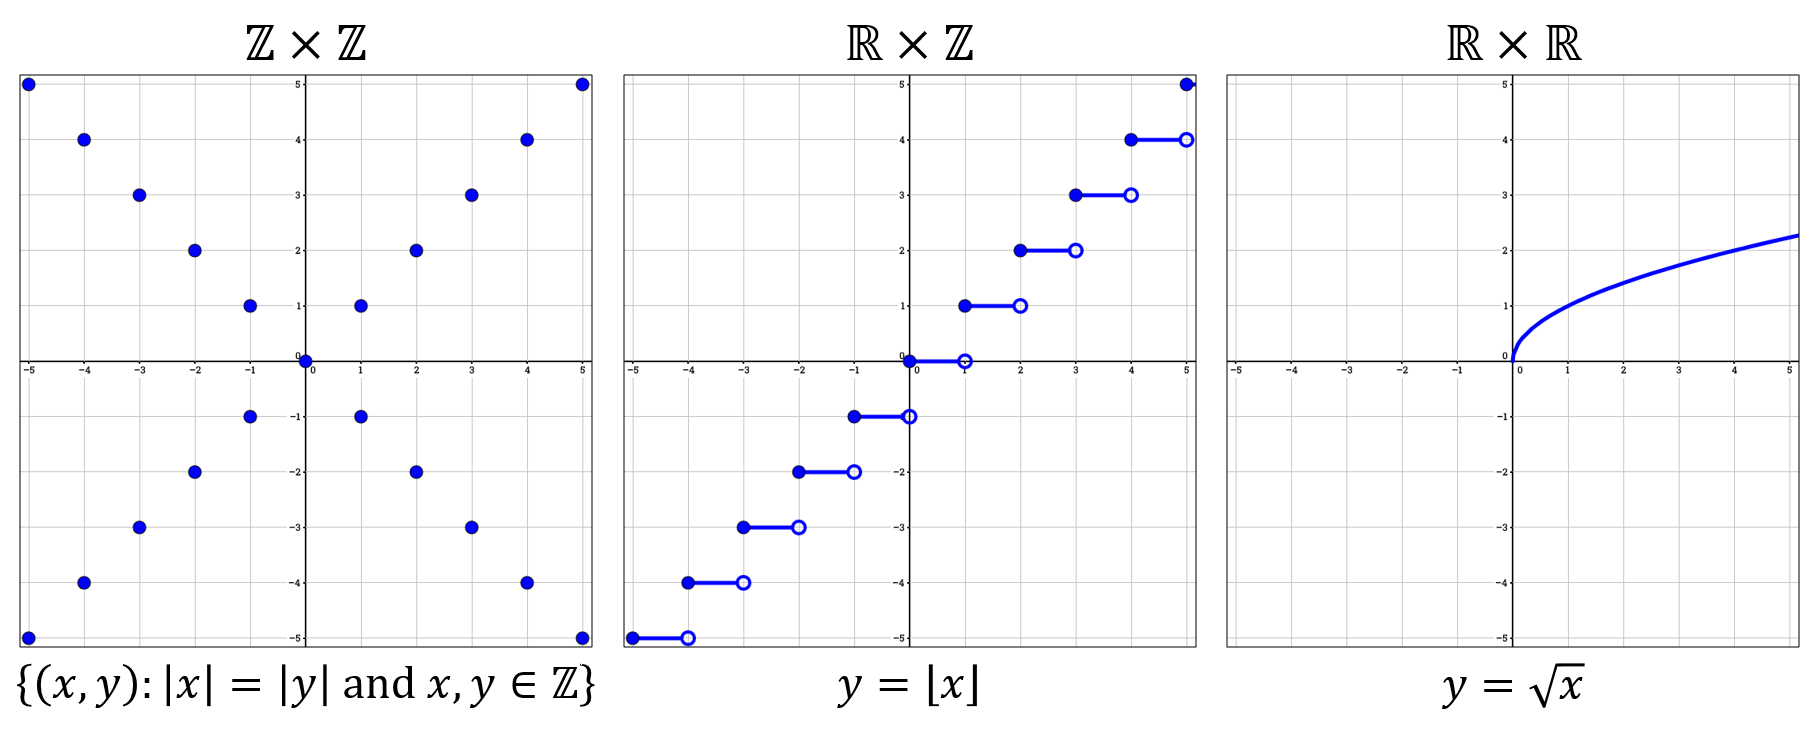
\includegraphics[width=5in]{images/graphrelations.png}
\caption{Graphs of relations. Constructed using GeoGebra}\label{fig:graphrelations}
\end{center}
\end{figure}

\begin{itemize}
\item
All three graphs are relations because all graphs are subsets of $A \times B$ (as specified at the top of each graph).
\item
The first and third relations are binary relations, but the second relation isn't because $A \neq B$.
\item
The first is not a function, because e.g. both $(1,1)$ and $(1,-1)$ are in the graph. 
The second is a function because it is uniquely defined on all of $A$ (in this case $A=\mathbb{R}$). The third is not a function because e.g. there is no pair of the form $(-1,y)$, so the function is not defined on all of $A$.
\end{itemize}
\end{example}

\begin{example}{ex_rel}
If $A = \{1,2,3\}$ and $B = \{4,5,6\}$, some examples of relations from $A$ to $B$ are:
\[ \{ (1,4), (2,5), (3,6)\}, \]
\[ \{ (1,6), (3,4)\}, \]
\[ \{ (2,5), (3,5) \}, \]
\[ \emptyset, \]
\[ \{ (1,4), (1,5), (1,6), (2,4), (2,5), (2,6), (3,4), (3,5), (3,6) \}.\] 
Notice that all of these sets are subsets of $A \times B$. The final example is the set $A \times B$ itself. Notice that $\emptyset$ is a valid relation because it's a subset of $A \times B$ (a subset with no elements).  On the other hand, the set $\{ \emptyset \}$ is \emph{not} a relation, because it is  a set with one element (namely $\emptyset$), and this element is not an element of $A \times B$. For similar reasons, $\{(1, \emptyset) \}$ is \emph{not} a relation.
\end{example}

\begin{example}{cities}
Let $A = \{\text{all cities in the U.S.}\}$ and $B = \{\text{all states in the U.S.}\}$. some examples of relations from $A$ to $B$ are:
\[ \{ \text{(Springfield,Illinois),(Springfield,Missouri),(Springfield,Texas),(Springfield,Wisconsin)}\}, \]
\[ \{ \text{(Corinth,Texas),(Liverpool,Texas),(Paris,Texas),(Sudan,Texas),(Troy,Texas)}\}, \]
\[ \{ \text{(Austin,Texas),(Boston,Massachusetts),(Phoenix,Arizona)}\}, \]
\[ \{ (x,y) \text{ such that } x \text{ is the capital of } y \}. \]
The third of these relations is a \emph{subset} of the last.
\end{example}


\begin{exercise}{7}
\begin{enumerate}[(a)]
\item
Let $A = \{a\}$ and $B = \{1\}$. List \emph{all} relations from $A$ to $B$.
\hyperref[secEqRelChapHints]{(*Hint*)}
\item
Let $A = \{a\}$ and $B = \{1,2\}$. List \emph{all} relations from $A$ to $B$.
\hyperref[secEqRelChapHints]{(*Hint*)}
\item
Let $A = \{a,b\}$ and $B = \{1\}$. List \emph{all} relations from $A$ to $B$.
\hyperref[secEqRelChapHints]{(*Hint*)}
\item
** Let $A = \{a,b\}$. List \emph{all} the binary relations on $A$.
\hyperref[secEqRelChapHints]{(*Hint*)}
\item
** Let $A = \{a,b,c\}$. How many binary relations are there on the set $A$?
\hyperref[secEqRelChapHints]{(*Hint*)}
\end{enumerate}
\end{exercise}

We'll mostly be concerned with binary relations, not relations from some set~$A$ to some other set~$B$.

\begin{exercise}{notbinary}
Let $S$ be the set of all living people. Which of the follow relationships define binary relations on $S$?
brother, pet, favorite color, dentist, college major, and professor?
 \end{exercise}

\begin{defn} \label{digraph} \index{Digraph}
We can draw a picture to represent any given binary relation on any given set~$A$:
	\begin{itemize}
	\item Draw a dot for each element of~$A$.
	\item For $a,b \in A$, draw an arrow from $a$ to~$b$ if and only if $(a,b)$ is an element of the relation.
	\end{itemize} 
The resulting picture is called a \term{digraph}. (The word is pronounced ``DIE-graff'' --- it is short for ``directed graph.''
\end{defn}
 
 \begin{example}{digraph1}
 Let $A =  \{1,2,3,4,5\}$. We can define a binary relation~$R_1$ on~$A$ by letting
 	\[ R_1 = \{\, (x,y) \mid x \neq y \text{ and } x^2 + y \leq 10 \,\} .\]
This binary relation is represented by the digraph in Figure~\ref{fig:x2y}:
\begin{figure}[htbp]
\begin{center}
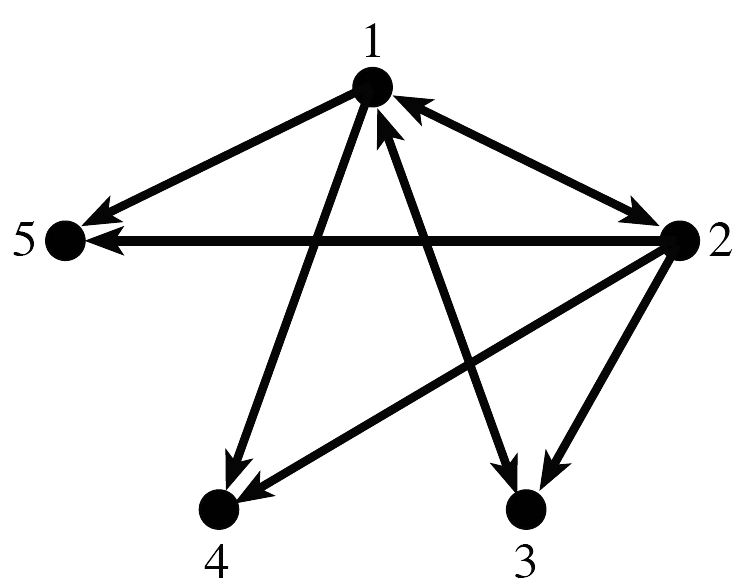
\includegraphics[width=3in]{images/x2+y.png}
\caption{Digraph of the binary relation of $R_1$}\label{fig:x2y}
\end{center}
\end{figure}

Note that there's a bidirectional arrow between $1$ and~$3$ because $(1,3) \in R_1$ and $(3,1) \in R_1$. On the other hand there's only a one directional arrow from $2$ to~$3$ because $(2,3) \in R_1$, but $(3,2) \notin R_1$.

We can also define a binary relation $R_2$ on $A$ by letting
$$R_2=\{(x,y) \text{ such that } x\mid y\},$$
where $x\mid y$ means $x$ divides $y$. This binary relation is represented by the digraph in Figure~\ref{fig:xdividesy}.
\begin{figure}[htbp]
\begin{center}
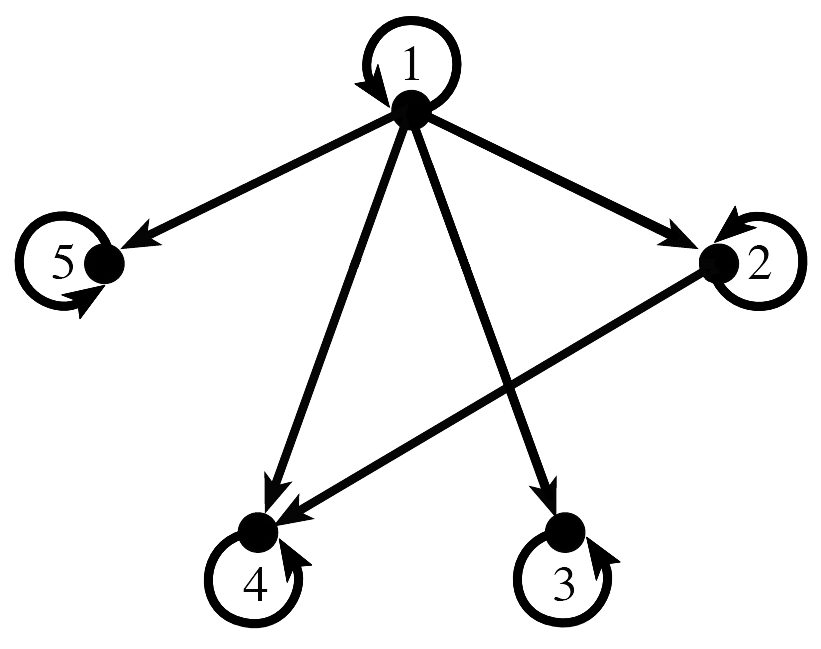
\includegraphics[width=3in]{images/xdividesy.png}
\caption{Digraph of the binary relation of $R_2$}\label{fig:xdividesy}
\end{center}
\end{figure}

In this digraph there are loops at each number because $a \mid a$ for each $a$.

\end{example}

 \begin{exercise}{DrawBinRelExer1}
Choose your favorite NBA team, and find a team roster (a good place to look is ESPN.com). Choose 6 players that have complete data, and let that be your set $A$.  draw a digraph for each of the following binary relations on~$A$: 
 \begin{enumerate}[(a)]
 \item \label{DrawBinRelExer-sister}
 $\{ (x,y) \in F \times F \,|\, x  \text{'s height is within 2 inches of }y\text{'s height} \}$
 \item \label{DrawBinRelExer-son}
 $\{ (x,y) \in A \times A \,|\, x\text{'s age is within the same decade as }y\text{'s}  \}$ 
 \item \label{DrawBinRelExer-married}
 The relation ``is taller than".
  \item \label{DrawBinRelExer-lived}
 The relation ``is less than 10 pounds heavier than".
 \end{enumerate}
 \end{exercise}
 
 \begin{exercise}{DrawBinRelExer3}
Let $A =  \{-2,-1,0,1,2\}$ Draw a digraph for each of the following binary relations on~$A$: 

 \begin{enumerate}[(a)]
 \item \label{DrawBinRelExer-son}
 $R_a = \{\, (x,y) \mid  x^2 = y^2 \,\} .$
 \item \label{DrawBinRelExer-sister}
$ R_b = \{\, (x,y) \mid  x^2 - y^2 < 2 \,\} .$
 \item \label{DrawBinRelExer-married}
 $ R_c = \{\, (x,y) \mid  (x-y)^2 < 2 \,\} .$
  \item \label{DrawBinRelExer-lived}
$ R_d = \{\, (x,y) \mid  x\equiv y \pmod{3} \,\} .$
 \end{enumerate}
 \end{exercise}

 \begin{exercise}{DrawBinRelExer2}
It is also possible to draw digraphs for relations that are not binary relations. In this case, your digraph should have a dot for each element of $A \cup B$.
% In each case, state whether or not your digraph is connected, and whether or not it is strongly connected.
 \begin{enumerate}[(a)]
 \item \label{DrawBinRelExer-son}
Draw digraph representations of the relations given in Example \ref{example:EquivalenceRelationsChap:ex_rel}.
 \item \label{DrawBinRelExer-sister}
The graphs you drew in (a) are all examples of \term{bipartite} graphs.  Complete the following definition:  A bipartite graph is a graph in which the vertices (dots) can be divided into two  sets, such that $\ldots$.
 \end{enumerate}
 \end{exercise}


We commonly use symbols  such as $=, < , \subset, \ldots $  that are used to compare elements of a set. You may have called these ``relations'' in your high school algebra class -- and in fact, they can all be considered as binary relations in the sense of Definition~\ref{relation}.
For example, using the symbol $<$ we can define the following binary relation on ${\mathbb R}$ :
\[ R_<  := \{\, (x,y) \in \mathbb{R} \times \mathbb{R} \mid x < y \}  \]
(here the symbol ``$:=$'' means ``defined as'').  Note that $ R_<$ here is a subset of $\mathbb{R} \times \mathbb{R}$, so it is indeed a binary relation according to Definition~\ref{relation}. 

% This book (like other mathematics textbooks) deals mainly with binary relations on sets of mathematical objects. In fact, you are quite familiar with many relations already. S

\begin{exer}\label{exercise:EquivalenceRelationsChap:RelationDef}
\begin{enumerate}[(a)]
 \item  
 Define the set $R_>$ associated with the symbol ``$>$'' applied to the natural numbers.
 \item  
 Define the set $R_=$ associated with the symbol ``$=$'' applied to the complex numbers. In your definition assume that equality of real numbers has been defined, and write complex numbers in rectangular form (for example, $a + bi$ or $c + di$).
 \item  
 List all the elements of the set $R_\subset$ associated with the symbol ``$\subset$'' applied to the subsets of $A := \{1,2\}$. (The set of subsets of $A$ is denoted as $\mathcal{P}(A)$, the \term{power set}\index{Power set} of $A$.)
 \hyperref[secEqRelChapHints]{(*Hint*)}
 \item  
Consider the set $R_\subset$ associated with the symbol ``$\subset$'' applied to the subsets of $A := \{1,2,3\}$. How many elements does $R_\subset$ have?
 \end{enumerate}
 \end{exer}
 
Exercise~\ref{exercise:EquivalenceRelationsChap:RelationDef} shows that any comparison symbol applied to a set gives rise to a binary relation. So rather than writing $R_<, R_>, R_=$ and so on, we simply use the comparison symbol itself to represent the binary relation.  Notice that technically, '$<$' defined on $\mathbb{R}$ is a different relation from '$<$' defined on $\mathbb{N}$: we will always make it very clear on which set the relation is being defined.

We will use the symbol $\rel$ (which may be read as ``is related to", ``tilde", or ``twiddle") to denote a generic comparison symbol. If we are working with the set $A$, then the symbol $\rel$ also represents the binary relation $A_\rel := \{\, (x,y) \in A \times A \mid x \rel y \}$.

We have shown that comparison symbols give rise to relations: the reverse is also true. Given a relation $R$ defined on the set $A$, we can define a comparison symbol $\rel$ applied to $a,b \in A$ as follows:
$ a \rel b$ iff $(a,b) \in R$.

\section{Partitions and properties of binary relations  \quad\sectionvideohref{SFk--oSOzfg&list=PL2uooHqQ6T7PW5na4EX8rQX2WvBBdM8Qo&index=18}} 
\label{sec:EquivalenceRelations:PartitionsAndProperties}

We've defined binary relations in general. In this section we present one very important situation where binary relations are very useful. It turns out that the binary relations which arise in this situation have some very special properties, which will become very important later.

Given any set $A$ with 2 or more elements, it's possible to split up the elements of $A$ into disjoint subsets. We call such a division a \term{partition}. The mathematical definition is:

\begin{defn}\label{def:Partition} A \term{partition}\index{Partition} $\mathcal{P}$ of a set~$A$ is a collection of nonempty subsets of~$A$, such that each element of~$A$ is in exactly one of the subsets in $\mathcal{P}$. In other words:
\begin{enumerate}[(a)]
\item the union of the subsets in $\mathcal{P}$ is all of~$A$,
and
\item the subsets in $\mathcal{P}$ are pairwise disjoint: that is the intersection of any two subsets is empty.\index{Partition!definition of}
\end{enumerate}
Conditions (a) and (b) imply that every element of $A$ is in exactly one subset in $\mathcal{P}$.
\end{defn}

\begin{rem}
Note that $\mathcal{P}$ is defined as a set of subsets of $A$. This means that the elements of $\mathcal{P}$ are \emph{subsets} which may contain multiple elements of $A$. The examples below with make this clearer.
\end{rem}

\begin{example}{partition1}
\begin{enumerate}[(a)]
\item Consider the set of real numbers $\mathbb{R}$. We know that every element of $\mathbb{R}$ belongs to one of two sets: the set of rational numbers, $\mathbb{Q}$, or the set of irrational numbers, $\mathbb{I}$. The union of these two subsets, $\mathbb{Q} \cup \mathbb{I}=\mathbb{R}$, and $\mathbb{Q}$ and $\mathbb{I}$ are disjoint sets, so based on the definition $\{\mathbb{Q},\mathbb{I}\}$ is a partition of $\mathbb{R}$. Alternatively the word ``partition" can be used as a verb, so we could also say that $\mathbb{Q}$ and $\mathbb{I}$ partition $\mathbb{R}$.
\item Let $\mathbb{E}$ and $\mathbb{O}$ be the even and odd integers, respectively. Then $\{\mathbb{E},\mathbb{O}\}$ is a partition of $\mathbb{Z}$. Alternatively we could also say that $\mathbb{E}$ and $\mathbb{O}$ partition $\mathbb{Z}$.
\item Let $S$ be the set of all single-element subsets of $\mathbb{Z}$, so that for example $\{-552\}$, $\{7\}$, $\{1492\}$ are all elements of $S$. Then $S$ is also a partition of $\mathbb{Z}$. Here $S$ has an infinite number of elements (all the single-element subsets of $\mathbb{Z}$), but each element of $S$ is a finite set.
\item Consider the set of complex numbers $\mathbb{C}$. Every element of $\mathbb{C}$ has a real part which we denote as Re$[z]$ (as in Chapter 2). Let $R_a$ be the set of all complex numbers with real part $a$, i.e. $R_a:=\{z \in \mathbb{C} \mid \text{Re}[z]=a\}$. Let $\mathcal{P}$ be the set consisting of all of the $R_a$'s, i.e. $\mathcal{P}:=\{R_a \forall a \in \mathbb{R}\}$. Then $\mathcal{P}$ is a partition of $\mathbb{C}$. Here $\mathcal{P}$ has an infinite number of elements, where each element of $\mathcal{P}$ is an infinite set.
\end{enumerate}
\end{example}

From the previous example you can see how partitions of sets of numbers are collections of subsets that divide up bigger sets. You could imagine it's like a little kid with a bucket of LEGO\textsuperscript{\textcircled{{\scriptsize R}}} bricks who's sorting them out into different piles. The LEGOs could be sorted by color, shape, number of studs, or the original set in which they were bought. Similarly there are lots of different ways to sort out sets of numbers, mathematical objects, or any arbitrary sets with elements of any kind. Each different way of sorting gives rise to a different partition.

\begin{example}{partition2}
\begin{enumerate}[(a)]
\item When making an inventory of the animals in a zoo, we may wish to count the number of antelopes, the number of baboons, the number of cheetahs, and so forth. In this case, all of the animals of the same species might be grouped together in a single set. Each species give rise to a different set and these sets form a partition of the animals in that zoo.
\item If we are concerned only with people's given names (what Americans would call ``first name"), we can partition any set of people according to given name. Each set in the partition consists of all people who share a particular given name.
\item In geometry, sometimes we are interested only in the shape of a triangle and not its location or orientation. In this case, we talk about \emph{congruent} triangles, where congruent means that corresponding sides of the two triangles are equal, and corresponding angles are also equal. For any triangle we may define the set of all triangles congruent to that triangle. There are an infinite number of such sets which form a partition of the set of all triangles.
\end{enumerate}
\end{example}


What do partitions have to do with relations? We will illustrate with the following example.

Let $A=\{1,2,3,4,5,6\}$ and partition these six numbers into evens and odds. Then we would have two subsets each with three elements. Suppose we use a six-sided die to determine a random outcome: where if we get an even number we win a dollar, but an odd number we lose a dollar. We don't care whether we get a 2, 4, or 6 -- only that we get an even number because we win the same amount regardless. In this way, rolling a 2, 4, or 6 are \emph{related}. Formally we can define a relation on $A$ as follows: Given $a,b \in A$, then $a \rel b$ iff $a$ and $b$ are either both even or both odd.

We generalize the previous example in the following definition. 

\begin{defn}\label{partitionrelation}
Given a partition $\mathcal{P}$ on $A$, we may define a binary relation $\rel_\mathcal{P}\,\subset A \times A$ as follows: for $a,b \in A$, $a \rel_\mathcal{P} b$ iff $a$ and $b$ are both contained in the same subset in the partition.
\end{defn}

We already know that binary relations can be represented graphically. In the following exercise, we investigate graphical representations of some binary relations that come from partitions.

\begin{exercise}{RelGraphR2}
In the following parts we will considering partitions of $\mathbb{R}$ and the associated binary relations defined by Definition~\ref{partitionrelation}. 
\begin{enumerate}[(a)]
\item Let $\mathcal{P}=\{R_1, R_2\}$ where $R_1=\{x \mid x \in \mathbb{R}, x \geq 0\}$ and $R_2=\{x \mid x \in \mathbb{R}, x < 0\}$.
\begin{enumerate}[(i)]
\item Draw the real number line from $-5$ to 5, and indicate the sets $R_1, R_2 \in \mathcal{P}$ (you may indicate the two sets by circling them separately).
\item Graph the associated binary relation $\rel_\mathcal{P}$. You only need to graph from $-5$ to 5. (Recall that the graph of a binary relation is a set in the Cartesian plane, as in Figure~\ref{fig:graphrelations}.)
\end{enumerate}

\item Let $\mathcal{P}=\{\ldots, R_{-2}, R_{-1}, R_0, R_1, R_2, \ldots \}$ where $R_n=\{x \mid x \in \mathbb{R}, \lfloor x \rfloor = n \}$ for any integer $n$. \footnote{The `L' brackets $\lfloor \cdots \rfloor$,  represent the \term{floor function}\index{Floor function}, also known as the greatest integer function. The floor function takes a real number, $x \in \mathbb{R}$ as input and outputs the greatest integer that is less than or equal to $x$.  For example: $\lfloor 4 \rfloor = 4$, $\lfloor \pi \rfloor = 3$, and $\lfloor -2.3 \rfloor = -3$.}
\begin{enumerate}[(i)]
\item Draw the real number line from $-5$ to 5, and indicate the visible sets in $\mathcal{P}$.
\item Graph the associated binary relation $\rel_\mathcal{P}$. You only need to graph from $-5$ to 5.
\end{enumerate}

\item Let $\mathcal{P}=\{\mathbb{E},\mathbb{O}\}$ where $\mathbb{E}=\{x \mid x \in \mathbb{R}, \lfloor x \rfloor \text{ is even}\}$ and $\mathbb{O}=\{x \mid x \in \mathbb{R}, \lfloor x \rfloor \text{ is odd}\}$.
\begin{enumerate}[(i)]
\item Draw the real number line from $-5$ to 5, and indicate the sets $\mathbb{E},\mathbb{O}  \in \mathcal{P}$  (a good way to do this is to color the intervals belonging to 
$\mathbb{E}$ and $\mathbb{O}$ with different colors).
\item Graph the associated binary relation $\rel_\mathcal{P}$. You only need to graph from $-5$ to 5.
\end{enumerate}
%\item possible exam question: x~y iff floor(abs(x)) = floor(abs(y)) or abs(floor(x)) = abs(floor(y))
\end{enumerate}
\end{exercise}

To further explore Definition~\ref{partitionrelation}, we let $A=\{a,b,c,\ldots,i\}$ which has been partitioned into subsets $A_1, \ldots, A_5$. Figure~\ref{fig:partition_discrete} has a drawing of $A$.

\begin{figure}[htbp]
\begin{center}
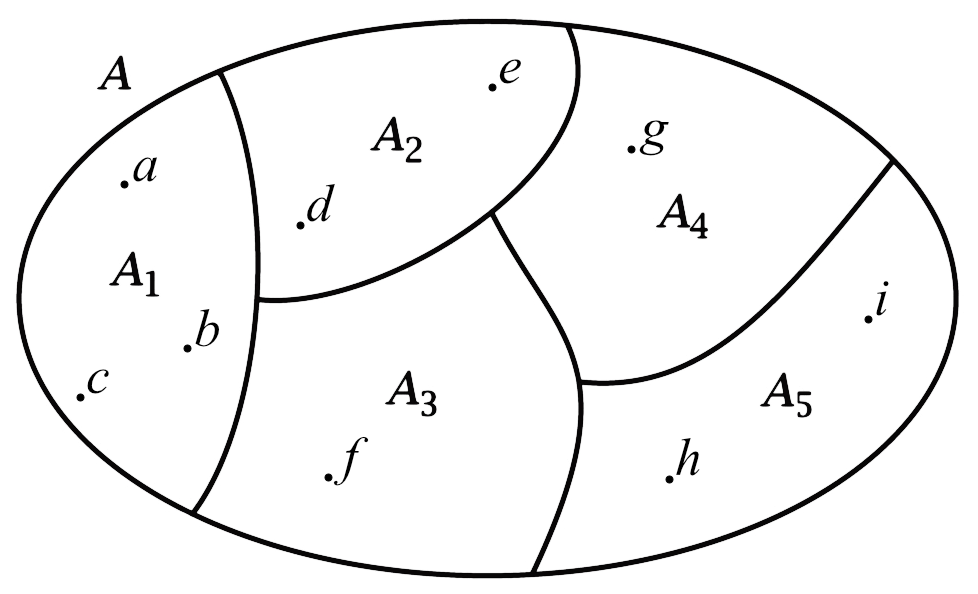
\includegraphics[scale=0.35]{images/partition_discrete.png}
\caption{A partition of~$A$ into subsets $A_1, \ldots, A_5$. 
(Each element of~$A$ is in one and only one of the subsets.)}\label{fig:partition_discrete}
\end{center}
\end{figure}

From Figure~\ref{fig:partition_discrete}, we can tell some properties of $\rel_\mathcal{P}$:
\begin{itemize}
\item Each element of $A$ is related to itself, that is:
$$a \rel_\mathcal{P} a$$
(this is called the \term*{reflexive}\index{Reflexive!property of relations}\index{Relation!reflexive}  property). 
We know this is true because $a$ is certainly in the same set of the partition as itself.
\item If an element is related to another element the relation also goes in the other direction. That is: 
$$a \rel_\mathcal{P} b \implies b \rel_\mathcal{P} a$$
(this is called the \term*{symmetric}\index{Symmetric!property of relations}\index{Relation!symmetric} property
We know this is true because if $a$ is related to $b$, then that means that $a$ and $b$ are in the same set of the partition. Since they are in the same set of the partition as each other $b$ is also related to $a$. This argument can easily be repeated in the other direction.
\item If an element is related to another element and that element is related to a third element, then the first element is related to the third. That is: 
$$a \rel_\mathcal{P} b \text{ and } b \rel_\mathcal{P} c \Rightarrow a \rel_\mathcal{P} c$$
(this is called the \term*{transitive} property\index{Transitive!property of relations}\index{Relation!transitive})
We know this is true because if $a$ is related to $b$ then they are in the same set of the partition, and if $b$ is related to $c$ then they too are in the same set of the partition. This means that $a$, $b$, and $c$ are all in the same set of the partition, therefore $a$ is related to $c$.
\end{itemize}

We have seen that the partition depicted in Figure~\ref{fig:partition_discrete} produces a binary relation with three distinctive properties. What about other partitions? Let's consider some of the partitions that we've defined previously.

\begin{example}{relfrompart1}
In this example we will define a binary relation from the given partition, and show that the relation has the above three properties.
\begin{enumerate}[(a)]
\item Given the partition in Example~\ref{example:EquivalenceRelationsChap:partition1}(a), we can define a binary relation $\rel_R$ on $\mathbb{R}$ by 
\[x \rel_R y  \text{   iff   }  (x,y \in \mathbb{Q} \text{ or }x,y \in \mathbb{I}).\]

\begin{itemize}
\item  First property (reflexive): $x \rel_R x$ ($x$ is always in the same set, $\mathbb{Q}$ or $\mathbb{I}$, as itself);
\item  Second property (symmetric): $x \rel_R y \implies y \rel_R x$ ($x$ is in the same set as $y$ implies $y$ is in the same set as $x$);
\item  Third property (transitive): $x \rel_R y$ and $y \rel_R z \eif x \rel_R z$ (if $x$ is in the same set as $y$ and $y$ is in the same set as $z$, then $x$ is in the same set as $z$);
\end{itemize}

\item Given the partition in Example~\ref{example:EquivalenceRelationsChap:partition2}(a), we can define a binary relation $\rel_S$ on the set of animals in the zoo by 
\[x \rel_S y  \text{   iff   }  x \text{ and } y \text{ are animals in the same species} .\]
\begin{itemize}
\item  Reflexive: $x \rel_S x$ ($x$ is always the same species as itself);
\item  Symmetric: $x \rel_S y \implies y \rel_S x$ ($x$ is the same species as $y$ implies $y$ is the same species as $x$);
\item  Transitive: $x \rel_S y$ and $y \rel_S z \eif x \rel_S z$ (if $x$ is the same species as $y$ and $y$ is the same species as $z$, then $x$ is the same species as $z$);
\end{itemize}
\end{enumerate}
\end{example}

\begin{exercise}{relfrompart2}
Define a binary relation from the given partition, and show that the relation has the above three properties.
\begin{enumerate}[(a)]
\item The partition in Example~\ref{example:EquivalenceRelationsChap:partition1}(b)
\item The partition in Example~\ref{example:EquivalenceRelationsChap:partition1}(c)
\item The partition in Example~\ref{example:EquivalenceRelationsChap:partition1}(d)
\item The partition in Example~\ref{example:EquivalenceRelationsChap:partition2}(b)
\item The partition in Example~\ref{example:EquivalenceRelationsChap:partition2}(c)
\end{enumerate}
\end{exercise}

The three properties seem to pop up whenever we define a binary relation from a patirtion. It's time to prove it.

\begin{prop}{partbinrel} Given a partition $\mathcal{P}$ on set $A$, define a binary relation of $A$ as $a \rel b$ iff there exists a subset $C \in \mathcal{P}$ such that $a$ and $b$ are both elements of $C$, then the binary relation, $\rel$, satisfies the following 3 properties:
\begin{enumerate}[(a)]
\item \term{reflexivity}:
	$$ \rel \text{ is reflexive} \iff \forall a \in A, a \rel a .$$\index{Relation!reflexive}\index{Reflexive}
\item  \term{symmetry}:
	$$ \rel \text{ is symmetric} \iff \bigl( \forall a,b \in A,  (a \rel b) \implies (b \rel a)\, \bigr)  .$$\index{Relation!symmetric}\index{Symmetric}
\item  \term{transitivity}:
	$$ \rel \text{ is transitive} \iff  \forall a,b,c \in A,  \bigl( (a \rel b) \mbox{ and } (b \rel c) \bigr) \eif (a \rel c)  .$$\index{Relation!transitive}\index{Transitive}
\end{enumerate}
\end{prop}

\begin{proof}
Earlier in the chapter we showed that the binary relation $\rel_\mathcal{P}$ from the partition in Figure~\ref{fig:partition_discrete} was reflexive, symmetric, and transitive. The arguments that we used are generally applicable, and can be used for any partition.
\end{proof}

\begin{rem} 
\begin{itemize}
\item In Proposition~\ref{proposition:EquivalenceRelationsChap:partbinrel} parts (a),(b), and (c) we used mathematical symbolism to express the concepts that were explained verbally in the discussion prior to Example~\ref{example:EquivalenceRelationsChap:relfrompart1}. Increasingly, you'll be expected to understand symbolism without verbal explanation. Here's a chance for you to practice: what does the following symbolism mean, and where have you seen it before? 
\[ a \sim b \quad \iff \quad \exists C \in \mathcal{P}, ( a \in C \text{ and } b \in C ) .\]
(Answer: this is the definition of  the relation $\sim$  defined in Proposition~\ref{proposition:EquivalenceRelationsChap:partbinrel}, expressed symbolically.
We'll be using this symbolism in later propositions, e.g. Proposition~\ref{proposition:EquivalenceRelationsChap:parteqrel}.) 

\item Even though the definition of symmetry begins with ``$\forall a,b \in A \ldots$" (``for every $a$ and $b$ in $A \ldots$") symmetry doesn't require \emph{every} pair of elements to be related to each other: symmetry only requires that whenever the \emph{if} clause ($a \rel b$) is true, the \emph{then} clause ($b \rel a$) must also be true. A similar caveat applies to transitivity.
\end{itemize}
\end{rem}

These properties  are so important that we have a special term for binary relations that satisfy all three properties:

\begin{defn}\label{defn:equivalencerelation}
An \term{equivalence relation}\index{Equivalence relation} on a set~$A$ is a binary relation on~$A$ that is reflexive, symmetric, and transitive.
\end{defn}

The following is a restatement of Proposition~\ref{proposition:EquivalenceRelationsChap:partbinrel}, using our new terminology.

\begin{prop}{parteqrel} Given a partition $\mathcal{P}$ on set $A$, define a binary relation $\sim$ on $A$ as follows: 
\[a \sim b \quad \iff \quad \exists C \in \mathcal{P}, ( a \in C \text{ and } b \in C ).\]  
Then the binary relation, $\rel$, is an equivalence relation.
\end{prop}

At one stroke, this proposition immediately proves that all  the relations defined from partitions in Examples~\ref{example:EquivalenceRelationsChap:partition1} and ~\ref{example:EquivalenceRelationsChap:partition2} are equivalence relations.

In the following sections we'll consider more examples of equivalence relations , but first let's make sure we understand reflexivity, symmetry and transitivity:

\begin{example}{binrelR} \ 
Consider the following binary relations on ${\mathbb R}$:
\begin{enumerate}[(a)]
\item $=$ is reflexive, symmetric, and transitive.
\begin{itemize}
\item 
Reflexive:  any real number $x$ equals itself, so $x=x~\forall x \in {\mathbb R}$.
\item
Symmetric:  for any real numbers $x$ and $y$, if $x = y$, then $y = x$. 
\item
Transitive:  for any real numbers $x$, $y$, and $z$, if $x = y$ and $y = z$, then $x = z$.
\item
Therefore $=$ on $\mathbb{R}$ is an equivalence relation because $=$ is reflexive, symmetric, and transitive.
\end{itemize}
\item $<$ is transitive, but neither reflexive nor symmetric.
\begin{itemize}
\item
Not Reflexive:  For example, it is not true that $1 < 1$.
\item
Not Symmetric:  For example, $1 < 2$ but it is not true that $2 < 1$.
\item
Transitive:  given three real numbers $x$, $y$, and $z$, if $x < y$ and $y < z$, then $x < z$.
\item
Therefore $<$ on $\mathbb{R}$ is not an equivalence relation.
\end{itemize}
\item
The binary relation $a \rel b$ iff $a = b + 1$ [for instance $(3.5,2.5) \in {\mathbb R}_\rel$] is neither reflexive, symmetric, or transitive.
\begin{itemize}
\item
Not Reflexive:  $3 \neq 3 + 1$.
\item
Not Symmetric:  $4 \rel 3$, since $4 = 3 + 1$, but $3 \not\rel 4$, since $3 \neq 4 + 1$.
\item
Not Transitive:  $4 \rel 3$ and $3 \rel 2$, but $4 \not\rel 2$ ($4 \neq 2 + 1$).
\item
Therefore $\rel$ when $a \rel b$ iff $a = b + 1$ on $\mathbb{R}$ is not an equivalence relation.
\end{itemize}  
\end{enumerate}
\end{example}

Notice that in the above examples, we used specific counterexamples to demonstrate when properties were not true.  We recommend that you do the same--and remember, it only takes \emph{one} counterexample to show a property is not true! 

\begin{exercise}{17}
For each of the following, explain your answers. 
\begin{enumerate}[(a)]
\item Is the binary relation $\leq$ defined on the set $\mathbb{R}$ reflexive? Is it symmetric? Is it transitive? Is it an equivalence relation?
\hyperref[secEqRelChapHints]{(*Hint*)}
\item Is  the binary relation $\subset$ defined on the set $\mathcal{P}(\mathbb{N})$ reflexive? Is it symmetric? Is it transitive? Is it an equivalence relation? (Recall that $\mathcal{P}(\mathbb{N})$ is the set of subsets of $\mathbb{N}$).
\item Define the binary relation $\rel$ on $\mathbb{C}$ as follows: $ z_1 \rel z_2$ iff $z_1 = |z_2|$. Is $\rel$ reflexive? Is it symmetric? Is it transitive? Is it an equivalence relation? \hyperref[secEqRelChapHints]{(*Hint*)} 
\item Define the binary relation $\rel$ on $\mathbb{Z}$ as follows: $ a \rel b$ iff $|a - b|< 4$. Is $\rel$ reflexive? Is it symmetric? Is it transitive? Is it an equivalence relation?
\end{enumerate}
\end{exercise}

\begin{example}{relonB}
Given the set $B = \{1,2,3\}$, consider the relation $\rel$ on $B$ defined by 
\[
B_\rel = \{(1,1), (2,2), (3,3), (1,2), (2,1), (2,3), (3,2) \}
\]
 The relation is shown in Figure~\ref{fig:relonB}.
\begin{figure}[htpb]
\begin{center}
 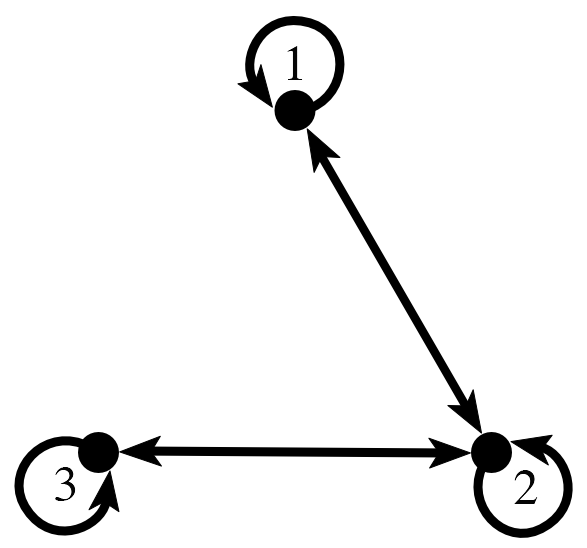
\includegraphics[width=2in]{images/relonB.png}
\caption{Diagram of the relation in Example~\ref{example:EquivalenceRelationsChap:relonB}\label{fig:relonB}}
\end{center}
\end{figure}

\begin{itemize}
\item $\rel$ is reflexive, because $1 \rel 1$, $2 \rel 2$, and $3 \rel 3$  (Note we had to check \emph{all} elements of the set $B$),
\item $\rel$ is symmetric, because, for each $(a,b) \in \mathord{\rel}$, the reversal $(b,a)$ is also in~$\rel$.
\item $\rel$ is \emph{not} transitive, because $1 \rel 2$ and $2 \rel 3$, but $1 \not\rel 3$.
\end{itemize}
\end{example}

Transitivity can sometimes be a little tricky, as the following examples show.

\begin{example}{transnotrefsym}
Let's think about binary relations on $\{1,2,3\}$ as seen in Figure~\ref{fig:transnotrefsym}. Which of the binary relations, A, B, or C, are transitive? Why or why not?

\begin{figure}[htpb]
\begin{center}
 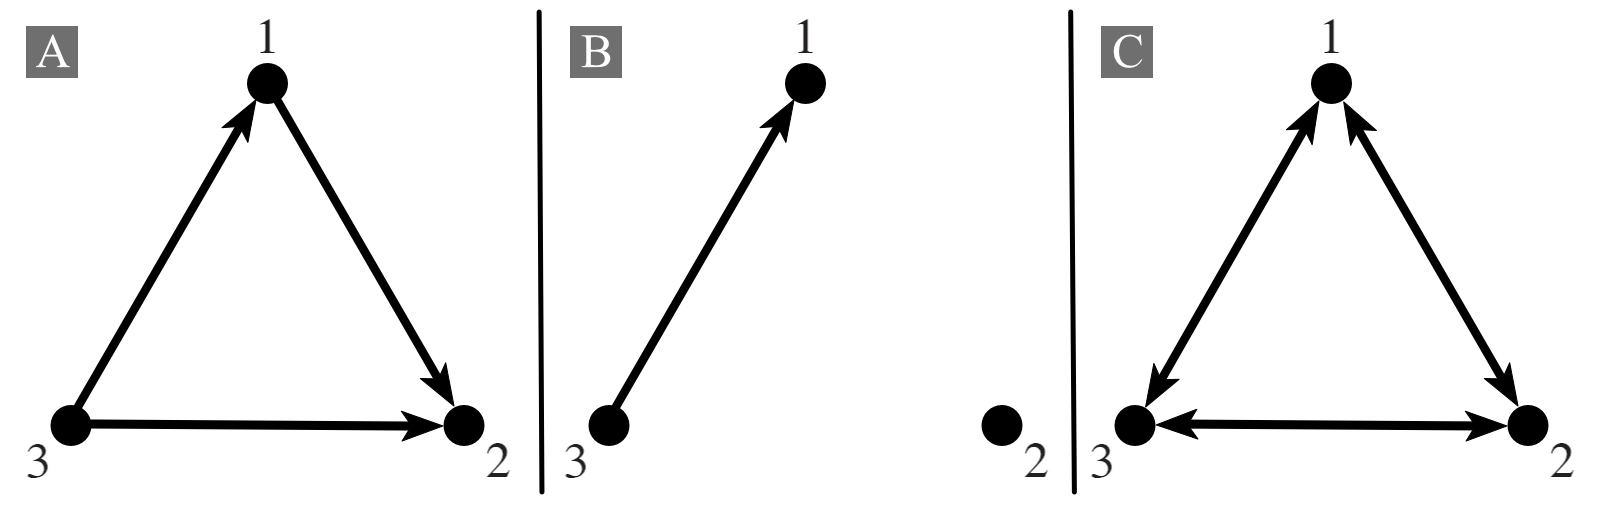
\includegraphics[width=5.5in]{images/transnotrefsym.png}
\caption{Digraphs to correspond with Example~\ref{example:EquivalenceRelationsChap:transnotrefsym}\label{fig:transnotrefsym}}
\end{center}
\end{figure}

Is  the relation in A transitive? Let's consider Remember how transitivity is defined:  if $a \rel b$ and $b \rel c$ then  $a \rel c$. In more prosaic terms, if there's an arrow from $a$ to $b$ and another arrow from $b$ to $c$, then there's an arrow directly from $a$ to $c$. We may conceptualize this as follows. Suppose $a$, $b$, and $c$ represent airports, and arrows represent flights between airports.  In terms of this example, transitivity means that whenever there's an indirect route between airports (with multiple stops), then there's also a direct route. So in the case of relation A, we may notice there's an indirect route from 3 to 2 by going through 1, but there's also a direct route from 3 to 2 (or more formally, $3 \rel 1$, $1 \rel 2$, and $3 \rel 2$). Furthermore this is the only example in A of an indirect route. Therefore this relation is transitive. If $3 \rel 2$ is removed from this binary relation, then the relation isn't transitive because it's still be possible to get from 3 to 2 via 1, but there's no longer a direct route.

How about the relation in digraph B?  This may be the most confusing of the bunch. One might think that B is not transitive, since there's only a single arrow--but think again. The definition of transitive says : \underline{\emph{ if}}  $a \rel b$ and $b \rel c$ then  $a \rel c$.  You may also read the ``if'' as ``whenever'':  \emph{Whenever}  $a \rel b$ and $b \rel c$ then it's also true that $a \rel c$.  But in relation B, the ``whenever'' \emph{never holds}, because there are no cases of $a \rightarrow b$ and $b\rightarrow c$  (i.e. there are no indirect routes).    This being the case, the ``if'' statement is considered true by default, so B is transitive.  This is an important point worth remembering: in mathematical logic, a statement is considered true if no counterexample exists. In other words, if you can \emph{prove} that there's no counterexample to a mathematical statement, then the statement is true! \footnote{Here are some ``true statements'', according to this rule :  (i) If you see a rainbow in the sky and follow it to where it touches the ground, you will find a leprechaun with a pot of gold; (ii) If you pick up an ordinary guinea pig by its tail, then its eyes will fall out. (iii) If you give a correct proof that 1=0, then Bill Gates will give you his entire fortune. }    
 

Lastly, the relation in digraph C is \emph{not} transitive. At first glance it seems like it should be transitive because so many transitivity conditions are satisfied (e.g. $1 \rel 2$ and $2 \rel 3 \Rightarrow 1 \rel 3$, etc), however we can also find transitivity conditions that fail (see part (a) of the following exercise)--and it only takes one counterexample to disprove a statement. 
\end{example}

\begin{exercise}{trickyTransitive}
\begin{enumerate}[(a)]
\item Give a counterexample that proves that the binary relation C in Figure~\ref{fig:transnotrefsym} is \emph{not} transitive. \hyperref[secEqRelChapHints]{(*Hint*)}
\item
Explain why the binary relation 
\[ R_{\sim} = \{(1,4), (1,1),(4,1) \} \]
is \emph{not} transitive.
\hyperref[secEqRelChapHints]{(*Hint*)} 
\item
Explain why the binary relation 
\[ R_{\sim} = \{(1,2), (1,3),(1,4) \} \]
\emph{is} transitive.
\hyperref[secEqRelChapHints]{(*Hint*)}
\end{enumerate}
\end{exercise}

\begin{exercise}{BinRelSomePropsEx}
Find binary relations on $\{1,2,3\}$ that meet each of the following conditions. Express each relation as a set of ordered pairs, and draw the corresponding digraph. (Note: each part can have more than one answer, but you only need to find one.)
\begin{enumerate}[(a)]
\item \label{BinRelSomePropsEx-symmonly}
symmetric, but neither reflexive nor transitive.
\item \label{BinRelSomePropsEx-refonly}
 reflexive, but neither symmetric nor transitive.
\item \label{BinRelSomePropsEx-transandsymm}
transitive and symmetric, but not reflexive.
\item \label{BinRelSomePropsEx-none}
neither reflexive, nor symmetric, nor transitive.
\end{enumerate}
\end{exercise}
Digraphs are useful because they represent the relation in such a way that it is easy to deduce the relation's properties: 

\begin{exercise}{21}
\begin{enumerate}[(a)]
\item
How can you tell from looking at a digraph whether or not the corresponding relation is reflexive?
\item
How can you tell from looking at a digraph whether or not the corresponding relation is symmetric? 
\item
**How can you tell from looking at a digraph whether or not the corresponding relation is transitive?
\end{enumerate}
\end{exercise}

%\section{Equivalence relations OLD} 
%\label{sec:EquivalenceRelations:EquivalenceRelationsOLD}

%\begin{rem}
%Each of the properties in \cref{RefSymmTransDefn} corresponds to a property of the digraph that we can draw of the relation. 
%\begin{itemize}
%\item A binary relation is reflexive if and only if the corresponding digraph has a loop at every vertex.
%\item A binary relation is symmetric if and only if every arc is in a digon in the corresponding digraph. (In such a case, we generally replace every digon by an edge and model the relation using a graph rather than a digraph.)
%\item A binary relation is transitive if and only if the corresponding digraph has the property that whenever one arc $\vec{uv}$ ends at the start of another arc~$\vec{vw}$, the arc $\vec{uv}$ is also in the digraph.
%\end{itemize}
%\end{rem}

%\begin{exer} \label{SymmTrans->ConnExer}
%Prove that if a binary relation is reflexive, symmetric, and transitive, then the corresponding graph has the property that any two vertices joined by a walk are adjacent. (That is, if there is a walk from~$u$ to~$v$, then $u$ is adjacent to~$v$.  In other words, every connected component of the graph is a complete graph with a loop at every vertex.)
%\hint{Use induction on $n$ to show that if there is a walk of length $n$ from~$u$ to~$v$ in the graph, then the edge $uv$ is in the graph.}
%\end{exer}

%\begin{exers} Suppose $\rel$ is a binary relation on a set~$A$.
%\begin{enumerate}
%\item Show that $\real$ is reflexive iff for all $a \in A$, we have $(a,a) \in \rel$.
%\end{enumerate}
%\end{exers}

%
%\begin{eg}
%Let $G$ be a simple graph with edge set $E$.
%Consider the relation $\sim$ defined on the vertex set of $G$ by $u \sim v \eiff uv \in E$.
%This relation:
%\begin{enumerate}
%\item is \emph{not} reflexive, because simple graphs are not allowed to have loops (edges from a vertex to itself);
%\item is symmetric, because if $uv \in E$ then $vu \in E$ is the same edge, looked at from the other end;
%\item may or may not be transitive, depending on the graph $G$.
%\end{enumerate}
%\end{eg}

%
%\begin{eg}
%Let $G$ be a simple digraph with arc set $A$.
%Consider the relation $\sim$ defined on the vertex set of $G$ by $u \sim v \eiff \vec{uv} \in A$.
%This relation:
%\begin{enumerate}
%\item is \emph{not} reflexive, because simple digraphs are not allowed to have loops (arcs from a vertex to itself);
%\item is symmetric only if every arc is part of a digon;
%\item may or may not be transitive, depending on the digraph $G$.
%\end{enumerate}
%\end{eg}

%\begin{exer} \label{EvenLengthRelExer}
% \ 
% \begin{enumerate}
%\item \label{EvenLengthRelExer-walk}
% Is the relation ``has a walk of even length" between two vertices of a graph reflexive? symmetric? transitive?  Justify your answers.
%\item \label{EvenLengthRelExer-path}
%  Is the relation ``has a path of even length" between two vertices of a graph reflexive? symmetric? transitive?  Justify your answers.
%\end{enumerate}
%\end{exer}

\section{Examples of equivalence relations\quad\sectionvideohref{ZtqFETtGm6o&list=PL2uooHqQ6T7PW5na4EX8rQX2WvBBdM8Qo&index=19}} 
 \label{sec:EquivalenceRelations:ExampleEquivRel}

Let's take a look at some examples of equivalence relations (recall Definition~\ref{defn:equivalencerelation}). We will see shortly that they all have something in common.

\begin{example}{binrelsquare}
Define a binary relation~$\sim$ on~$\real$ by $x \sim y$ iff $x^2 = y^2$. Then $\sim$ is an equivalence relation.

\begin{proof}
We wish to show that $\sim$ is reflexive, symmetric, and transitive.

\noindent
(reflexive) Given $x \in \real $, we have $x^2 = x^2$, so $x \sim x$.

\noindent
(symmetric) Given $x,y \in \real$, such that $x \sim y$, we have $x^2 = y^2$. Since equality is symmetric, this implies $y^2 = x^2$, so $y \sim x$.

\noindent
(transitive) Given $x,y,z \in \real$, such that $x \sim y$ and $y \sim z$, we have $x^2 = y^2$ and $y^2 = z^2$. Therefore $x^2 = z^2$, since equality is transitive. Hence $x \sim z$.
\end{proof}
\end{example}


%\begin{eg}
%For any $n \in \integer$, we know that congruence modulo~$n$ is reflexive, symmetric, and transitive (see \cref{CongEquivRel}). Therefore, congruence modulo~$n$ is an equivalence relation.
%\end{eg}


\begin{example}{NxNEquivRelEg}
Define a binary relation~$\sim$ on~$\mathbb{N} \times \mathbb{N}$ by $(a_1,b_1) \sim (a_2,b_2)$ iff $a_1 + b_2 = a_2 + b_1$. Then $\sim$ is an equivalence relation.

\begin{proof}
We wish to show that $\sim$ is reflexive, symmetric, and transitive.

\noindent
(reflexive) Given $(a,b) \in \mathbb{N} \times \mathbb{N}$, we have $a + b = a + b$, so $(a,b) \sim (a,b)$.

\noindent
(symmetric) Given $(a_1,b_1) , (a_2,b_2) \in \mathbb{N} \times \mathbb{N}$, such that $(a_1,b_1) \sim (a_2,b_2)$, we have $a_1 +b_2 = a_2 + b_1$. Since equality is symmetric, this implies $a_2 + b_1 = a_1 + b_2$, so $(a_2,b_2) \sim (a_1,b_1)$.

\noindent
(transitive) Given $(a_1,b_1) , (a_2,b_2) , (a_3,b_3) \in \mathbb{N} \times \mathbb{N}$, such that $(a_1,b_1) \sim (a_2,b_2)$ and $(a_2,b_2) \sim (a_3,b_3)$, we have 
	\begin{align*}
	(a_1 + b_3) + (a_2 + b_2)
		&= (a_1 + b_2) + (a_2 + b_3) && \text{(rearrange terms)}
		\\&= (a_2 + b_1) + (a_2 + b_3) && (\,(a_1,b_1) \sim (a_2,b_2)\text{ and substitution})
		\\&= (a_2 + b_1) + (a_3 + b_2) && (\,(a_2,b_2) \sim (a_3,b_3)\text{ and substitution})
		\\&= (a_3 + b_1) + (a_2 + b_2) && \text{(rearrange terms)} .
	\end{align*}
Subtracting $a_2 + b_2$ from both sides of the equation, we conclude that $a_1 + b_3 = a_3 + b_1$,
so $(a_1,b_1) \sim (a_3,b_3)$.
\end{proof}
\end{example}


\begin{exercise}{EquivRelShowEx}
Show that each of these binary relations is an equivalence relation.
\begin{enumerate}[(a)]
\item \label{EquivRelShowEx-x2min3x}
The binary relation $\sim$ on $\real$ defined by $x \sim y$ iff $x^2 - 3x = y^2 - 3y$.
\item \label{EquivRelShowEx-xminyinZ}
The binary relation $\sim$ on $\real$ defined by $x \sim y$ iff $x - y \in \integer$.
\hyperref[secEqRelChapHints]{(*Hint*)}
\item \label{EquivRelShowEx-ab=ab}
The binary relation $\sim$ on $\mathbb{N} \times \mathbb{N}$ defined by $(a_1,b_1) \sim (a_2,b_2)$ iff $a_1 b_2 = a_2 b_1$.
\hyperref[secEqRelChapHints]{(*Hint*)}
\item \label{EquivRelComplex1}
The binary relation $\sim$ on $\mathbb{C}$ defined by $z_1 \sim z_2$ iff $|z_1|=|z_2|$.
\item \label{EquivRelComplex1}
The binary relation $\sim$ on $\mathbb{C}$  defined by $z_1 \sim z_2$ iff Re[$z_1$] = Re[$z_2$].  (Recall that Re[$z$] is the real part of $z$)
\item
The binary relation $\sim$ on the collection of all finite sets defined by
\[  A \sim B  \text{ iff } |A|=|B|  \text{  (that is, }A \text{ and } B \text{ have the same number of elements)} \]
\end{enumerate}
\end{exercise}


Equivalence relations are often defined in terms of \emph{functions}.  For instance,  Example~\ref{example:EquivalenceRelationsChap:binrelsquare}  involves the function $f: \mathbb{R} \rightarrow 
\mathbb{R}$ defined by $f(x)=x^2$, and $x \sim y$ if and only if $f(x) = f(y)$.  Similarly, Exercise~\ref{exercise:EquivalenceRelationsChap:EquivRelShowEx} involves the function 
$g: \mathbb{R} \rightarrow 
\mathbb{R}$ defined by $f(x)=x^2-3x$, and $x \sim y$ if and only if $g(x) = g(y)$.
Both of these cases follow the following pattern:

\begin{equation*}
\mbox{Given a function $f: A \rightarrow B$, define a binary relation on $A$ by: $a_1 \rel a_2$ iff $f(a_1) = f(a_2)$.}
\end{equation*}

Other examples that we've seen also follow this same pattern:

\begin{exercise}{pattern}
Following the pattern that we've shown for Example~\ref{example:EquivalenceRelationsChap:binrelsquare}  and Exercise~\ref{exercise:EquivalenceRelationsChap:EquivRelShowEx},
define the following equivalence relations in terms of functions.
\begin{enumerate}[(a)]
\item
Exercise~\ref{exercise:EquivalenceRelationsChap:EquivRelShowEx} part (d) 
\item
Exercise~\ref{exercise:EquivalenceRelationsChap:EquivRelShowEx} part (e) 
\item
The binary relation in   Example~\ref{example:EquivalenceRelationsChap:NxNEquivRelEg}.
\end{enumerate}
\end{exercise}


The previous examples have all involved sets of numbers, but we may see that the same thing happens even when we consider functions on other types of sets.

\begin{example}{MoreEquivRelEgs}
\begin{enumerate}[(a)]
\item Every animal has only one species, so $\var{Species}$ is a function that is defined on the set of all animals. The equivalence relation~$\rel_S$ of Example~\ref{example:EquivalenceRelationsChap:relfrompart1} can be characterized by
\[ x \rel_S y \quad \iff \quad {\var Species}(x) = {\var Species}(y) .\]
\item If we assume that every person has a given name, then $\var{GivenName}$ is a function on the set of all people. Let $\rel_N$ be the equivalence relation of Exercise~\ref{exercise:EquivalenceRelationsChap:relfrompart2} can be characterized by
\[  x \rel_N y \quad \iff \quad {\var GivenName}(x) = {\var GivenName}(y) .\]
\end{enumerate}
\end{example}

We've given enough examples to (hopefully) convince you that functions always produce equivalence relations. But examples are never enough! The bottom line is that we need a proof--and here it is.

\begin{prop}{EquivRelFromFunc}
Suppose $f \colon A \to B$. If we define a binary relation~$\sim$ on~$A$ by
\[ a_1 \sim a_2 \quad \iff \quad f(a_1) = f(a_2) ,\]
then $\sim$ is an equivalence relation on $A$.
\end{prop}

\begin{exercise}{EquivRelFromFuncPfEx}
Prove Proposition~\ref{proposition:EquivalenceRelationsChap:EquivRelFromFunc}: that is, prove that the relation defined in the proposition is (a) reflexive, (b) symmetric, and (c) transitive.  (If you like, you may model your proof on the discussion prior to Exercise~ Example~\ref{example:EquivalenceRelationsChap:relfrompart1}, where we proved the three properties for binary relations arising from partitions.)

\end{exercise}

Let's take a step back and take stock of where we are. We've shown (Proposition~\ref{proposition:EquivalenceRelationsChap:partbinrel}) that any partition has an associated equivalence relation. We've also shown (Proposition~\ref{proposition:EquivalenceRelationsChap:EquivRelFromFunc}) that any function has an associated equivalence relation. Is there any relationship between these two facts? Indeed, we'll see in subsequent discussions that partitions, functions, and equivalence relations are closely interrelated. In the following exercise, we'll show that any equivalence relation that comes from a partition also comes from a function.

\begin{exercise}{partitionfunction}
Given a set $A$ and a partition $\mathcal{P}=\{A_1, A_2, A_3, \ldots\}$ of $A$.  Let $\rel_\mathcal{P}$ be the equivalence relation associated with the partition $\mathcal{P}$. Now define a function $f:A \rightarrow \mathbb{N}$ as follows:

$$f(a)=
\begin{cases}
1 & \mbox{if $a \in A_1$} \\
2 & \mbox{if $a \in A_2$} \\
\vdots & \vdots \\
n & \mbox{if $a \in A_n$}
\end{cases}$$

In general: $f(a)=j$ iff $a \in A_j$.
\begin{enumerate}[(a)]
\item
Show that $a \rel_\mathcal{P} b \iff f(a)=f(b)$.
\item 
Let $\rel_f$ be the equivalence relation defined from $f$ as in Proposition~\ref{proposition:EquivalenceRelationsChap:EquivRelFromFunc}. 
Show that $\rel_\mathcal{P} = \rel_f$ by showing that $a \rel_\mathcal{P} b \iff a \rel_f b$.
\end{enumerate}
\end{exercise}

Exercise~\ref{exercise:EquivalenceRelationsChap:partitionfunction} amounts to a proof of the following proposition.     

\begin{prop}{PartToFunc}
Given a set $A$ with partition $\mathcal{P}=\{A_1, A_2, A_3, \ldots \}$. 
Let $\rel_{\mathcal{P}}$ be the associated equivalence relation. 
Then there exists a function $f:A \rightarrow \mathbb{N}$ with associated equivalence relation $\rel_f$ such that 
$\rel_{\mathcal{P}} \, = \, \rel_{f}$.
\end{prop}

In other words, whenever we have a partition, we can also define a function that gives us the same equivalence relation as the partition.
\footnote{This statement is true, but the proof in Exercise~\ref{exercise:EquivalenceRelationsChap:partitionfunction} isn't quite complete. The reason is that we've assumed that the partition $\mathcal{P}$ is \term{countable}, i.e. we can assign a unique natural number index to each set in $\mathcal{P}$. There are many sets in mathematics that are \emph{not} countable (such as the real numbers). To make a truly general proof, we should specify an index set that may depend on the partition.}

%Notice that the previous proposition is not an if and only if proposition, because there could be an equivalence relation that can't be expressed as a function. But the good news about this proposition is that many relations can be expressed as a function as the previous examples and exercises have shown, including functions with arbitrary sets.

\begin{exercise}{realfunction}
From the relation $\rel_R$ in Examples~\ref{example:EquivalenceRelationsChap:partition1}(a) and~\ref{example:EquivalenceRelationsChap:relfrompart1}(a) (the $\mathbb{Q}$ and  $\mathbb{I}$ example) define a function such that $a_1 \sim a_2 \iff  f(a_1) = f(a_2)$ where $a_1, a_2 \in \mathbb{R}$.  (Note that we've already proved that $\rel_R$ is an equivalence relation by a different proposition, so this example is a particular case of Proposition~\ref{proposition:EquivalenceRelationsChap:PartToFunc}.) 
\end{exercise}

Exercise~\ref{exercise:EquivalenceRelationsChap:partitionfunction} starts with a partition, and constructs a function that gives the same equivalence relation as the partition.  We may go backwards as well: starting with a function, we may produce a partition with the same equivalence relation. The following exercise gives an example of this.

\begin{exercise}{66}
Let $f\colon \{-3,-2,-1,0,1,2,3\} \to \mathbb{Z}$ be defined by $f(x) =  x^2$.
\begin{enumerate}[(a)]
\item
What is the range of $f$?
\item
For every number $n$ in the range of $f$, find the set of all numbers in the domain of $f$ that map to $n$. Denote this set as $A_n$ (for example, if we let $n=0$, then only 0 maps to 0, so $A_0 = 0$). List the elements of $A_n$ for each $n$ in the range of $f$. 
\item 
Show that the sets $\{ A_n \}$ that you listed in part (b) form a partition of the domain of $f$.
\item
According to Proposition~\ref{proposition:EquivalenceRelationsChap:EquivRel->Part}, this partition produces an equivalence relation  on  the domain of $f$.  Draw a digraph that represents the equivalence relation.
\item
We also know that the function $f$ produces an equivalence relation on the domain of $f$, as in Proposition~\ref{proposition:EquivalenceRelationsChap:EquivRelFromFunc}.  Draw a digraph that represents this equivalence relation.
\item
What may you conclude from your results in (d) and (e)?   
\end{enumerate}
\end{exercise}

The following proposition generalizes the results of the previous exercise.

\begin{prop}{FuncIsRange}
Suppose $f:A \rightarrow B$. For each $b \in \text{Range}(f)$ define a subset $A_b \subset A$ as follows:
$$A_b:=\{a \in A \mid f(a)=b \}.$$
Then the collection of sets $ \mathcal{P} :=\{A_b \, |\,  b \in B\}$ form a partition of $A$. Furthermore, the equivalence relation $\sim_f$ derived from $f$ is identical to the equivalence relation $\sim_{\mathcal{P}}$ derived from $\mathcal{P}$: that is, $a_1 \sim_f a_2 \iff a_1 \sim_{\mathcal{P}} a_2$.
\end{prop}
\begin{proof}  The proof is broken up into steps in the following exercise.

\begin{exercise}{Abdisjoint}
\begin{enumerate}[(a)]
\item Given any $b \in \text{Range}(f)$, show that $A_b$ is nonempty
\item Given $b_1, b_2\in \text{Range}(f)$ with $b_1 \neq b_2$, show that $A_{b_1}$ and $A_{b_2}$ are disjoint, i.e. $A_{b_1} \cap A_{b_2}=\emptyset$.  
\item Given any $a \in A$, show there exists a $b \in \text{Range}(f)$ such that $a \in A_b$. 
\item Show that $\{A_b \, | \, b \in B\}$ includes all of $A$; that is, $A=\cup_{b \in B} A_b$.
\item Verify that the (a)-(d) imply that $\{A_b | b \in B\}$ is a partition of $A$.
\end{enumerate}
\end{exercise}
\end{proof}

\section{Obtaining partitions from equivalence relations\quad\sectionvideohref{LGU0Dhcozr8&list=PL2uooHqQ6T7PW5na4EX8rQX2WvBBdM8Qo&index=20}} \label{sec:EquivalenceRelations:ObtainingPartitions}

Proposition~\ref{proposition:EquivalenceRelationsChap:parteqrel} tells us that given any partition $\mathcal{P}$ of a set $S$, we can define an equivalence relation which says that two elements of $S$ are equivalent iff they belong to the same set in the partition. We'll see in this section that we can go the other way as well: namely, given any equivalence relation on $S$ we can construct a partition on $S$ which divided all the elements of $S$ among disjoint subsets.

To make this work, we first must define a key notion: \emph{equivalence classes}. Here we go!

 \subsection{From equivalence relations to equivalence classes}

Let's ramp up to our key definition by means of  an example. 

\begin{example}{}
Suppose we're studying a set of people, and we're only interested in their given names.  Of course there may be several Johns, several Marys, a couple of Sylvesters, and so on-- but  as far as given names are concerned, any two Johns can be considered as equivalent: indeed, we formalized this sense of equivalence in Example~\ref{example:EquivalenceRelationsChap:MoreEquivRelEgs}(b). We can group all Johns into a single set or class, which we'll refer to as an  \emph{equivalence class}. We can do the same thing with Marys, Sylvesters, Xyleenas, Zenobias, and so on. It follows that every person in the set belongs to her or his own equivalence class (even if the equivalence class consists of a single person!)
\end{example}

Let's generalize this example. Essentially, the only fact about given names that we used to define equivalence classes was that given name defines an equivalence relation on the set of interest. So it stands to reason that we can do something similar with any equivalence relation:
 
 \begin{defn}\label{DefEquivRel}
 Suppose $\sim$ is an equivalence relation on a set~$A$. For each $a \in A$, the \term{equivalence class}\index{Equivalence class} of~$a$ is the following subset of~$A$:
 	$$ [a] = \{\, s \in A \mid s \sim a \,\} .$$
That is, the equivalence class of the element $a \in A$ is the set of all elements of $A$ that are equivalent to $a$.
\end{defn}


\begin{example}{}
For the equivalence relation~$N$ described in Example~\ref{example:EquivalenceRelationsChap:MoreEquivRelEgs}(b), we have
	$$ [\var{Woodrow\,\,Wilson}] = \{\, x \in \var{People} \mid \var{GivenName}(x) = \var{GivenName}(\var{Woodrow\,\,Wilson}) \,\} .$$
In other words, $[\var{Woodrow\,\,Wilson}]$ is the set of all people whose given name is Woodrow.
\end{example}

\begin{warn}
The notation $[a]$ does not tell us which equivalence relation is being used. You should be able to figure out which relation it is from the context.
\end{warn}

Let's give a a more ``mathy'' example.

\begin{example}{EquivClassEg}
Suppose $A = \{1,2,3,4,5\}$ and 
\begin{align*}
&R = \\
&\left\{  (1,1), (1,3), (1,4), (2,2), (2,5), (3,1), (3,3), 
		(3,4), (4,1), (4,3), (4,4), (5,2), (5,5) 
\right\}
\end{align*}
One can verify that $R$ is an equivalence relation on~$A$. The equivalence classes are:
$$ [1] = [3] = [4] = \{1,3,4\},
\quad [2] = [5] = \{2,5\}.$$
\end{example}

\begin{exercise}{EquivClassEasyEx}
\begin{enumerate}[(a)]
\item \label{EquivClassEasyEx-set}
Let $B = \{1,2,3,4,5\}$ and 
	$$S = \left\{ (1,1),\, (1,4),\, (2,2),\, (2,3),\, (3,2),\, 
		(3,3),\, (4,1),\, (4,4),\, (5,5)
		 \right\} .$$
Assume (without proof) that $S$ is an equivalence relation on~$B$. Find the equivalence class of each element of~$B$.


\item \label{EquivClassEasyEx-x+y}
Let $C = \{1,2,3,4,5\}$ and define $\rel_C$ by 
\[ x \rel_C y \iff x + y \text{ is even.} \]
Assume (without proof) that $\rel_C$ is an equivalence relation on~$C$. Find the equivalence class of each element of~$C$.
\item
Draw the arrow diagrams for the relations in $R$ in Example~\ref{example:EquivalenceRelationsChap:EquivClassEg}, and for the relations in parts ($a$) and ($b$) of this exercise.
\end{enumerate}
\end{exercise}


The following proposition presents some very important properties of equivalence classes:

\begin{prop}{EquivRelProps}
Suppose $\sim$ is an equivalence relation on a set~$S$. Then:
\begin{enumerate}[(a)]
\item \label{EquivRelProps-aIn[a]}
 For all $a \in S$, we have $a \in [a]$.
\item \label{EquivRelProps-nonempty}
 For all $a \in S$, we have $[a] \neq \emptyset$.
\item \label{EquivRelProps-union}
 The union of the equivalence classes is all of~$S$. This can be written mathematically as follows:
	$$ \bigcup_{a \in S} [a] = S$$
%Every element of~$S$ is in some equivalence class.
\item \label{EquivRelProps-equal}
 For any $a_1,a_2 \in S$, such that $a_1 \sim a_2$, we have $[a_1] = [a_2]$.
\item \label{EquivRelProps-disjoint}
 For any $a_1,a_2 \in S$, such that $a_1 \not\sim a_2$, we have $[a_1] \cap [a_2] = \emptyset$.
\end{enumerate}
\end{prop}

\begin{exercise}{EquivRelPropsPfEx}
Prove the assertions in Proposition~\ref{proposition:EquivalenceRelationsChap:EquivRelProps}. You may use the following hints:
\begin{enumerate}[(a)]
\item
Use the reflexive property of $\sim$, together with Definition~\ref{DefEquivRel}
\item
Use part (a).
\item
This can be done by showing:
\begin{enumerate}[(i)]
\item 
$\bigcup_{a \in S} [a] \subset S$
\item
$S \subset \bigcup_{a \in S} [a]$
\end{enumerate}
In (i), use the fact that $[a] \subset S$.  In (ii), use (a) above to show that every element of $S$ is in at least one equivalence class. (Recall also that `$\subset$' means ``contained in'', and  includes the case where the two sets are equal.)
\item
Remember that two sets are equal if they have all their elements in common. So you want to show that given $a_1 \rel a_2$, then every element of $[a_1]$ is also an element of [$a_2]$, and vice versa. Do this as follows: 
\begin{itemize}
\item
Choose any $a_3 \in [a_1]$. Use Definition~\ref{DefEquivRel} together with the transitive property to show that $a_3 \in [a_2]$. Conclude that every element of $[a_1]$ is also an element of $[a_2]$. 
\item
Use a similar proof to show that every element of $[a_2]$ is also an element of $[a_1]$.
\end{itemize}
\item
You can prove this one by contradiction. Suppose the intersection is non-empty. Choose an element in the intersection. Use Definition~\ref{DefEquivRel} and the transitive property to derive a contradiction.
\end{enumerate}
\end{exercise}

Proposition~\ref{proposition:EquivalenceRelationsChap:EquivRelProps} also gives us this important fact:

\begin{prop}{DisjointEquiv}
Suppose $\sim$ is an equivalence relation on a set~$S$. Then any two equivalence classes are either equal or disjoint; that is, either they have exactly the same elements, or they have no elements in common. 
\end{prop}

\begin{exercise}{DisjointEquivEx}
Fill in the blanks to complete the proof of Proposition~\ref{proposition:EquivalenceRelationsChap:DisjointEquiv}:

\begin{proof}
It's enough to show that any two equivalence classes $[a_1]$ and~$[a_2]$ that are not disjoint must in fact be equal. \index{Disjoint!applied to equivalence relations}
\begin{enumerate}[(a)]
\item
Since the equivalence classes are not disjoint, their intersection is nonempty: so there is some $a \in [a_1] \cap \_\_\_\_\_\_\_\_$. 
\item
Hence, $a \in \_\_\_\_\_\_\_\_$ and $a \in \_\_\_\_\_\_\_\_$. 
\item
By Definition~\ref{DefEquivRel}, this means $a \sim \_\_\_\_\_\_\_\_$ and $a \sim \_\_\_\_\_\_\_\_$. 
\item
Hence, Proposition~\ref{proposition:EquivalenceRelationsChap:EquivRelProps} part \_\_\_\_\_\_\_\_  tells us that $[a] =\_\_\_\_\_\_\_\_$ and $[a] =\_\_\_\_\_\_\_\_$. 
\item
Therefore $\_\_\_\_\_\_\_\_ = [a] = \_\_\_\_\_\_\_\_$, as desired.
\end{enumerate}
\end{proof}
\end{exercise}

\subsection{From equivalence classes to partitions}

It's time to come full circle, and show that partitions arise from equivalence classes. As in the previous section, we'll ramp up with an example.

\begin{example}{EquivClassPartEg}
In Example~\ref{example:EquivalenceRelationsChap:EquivClassEg}, the equivalence classes are $\{1,3,4\}$ and $\{2,5\}$. Since $1,2,3,4,5$ each belong to exactly one of these sets, we see that the set
	$$ \bigl\{ \{1,3,4\}, \{2,5\} \bigr\} $$
of equivalence classes is a partition of $\{1,2, 3,4,5\}$.
\end{example}

Intuitively, equivalence classes resulting from an equivalence relation on $S$ will always break $S$ up into disjoint sets which, taken together, include all the elements of $S$. We've seen this description before--this is exactly what a partition does. This observation places us at the doorstep of the following proposition:

\begin{prop}{EquivRel->Part}
Suppose $\sim$ is an equivalence relation on a set~$A$. Then 
	$$ \{\, [a] \mid a \in A \,\} $$
is a partition of~$A$.
\end{prop}

\begin{proof}
From parts (\ref{EquivRelProps-nonempty}), (\ref{EquivRelProps-union}), and (\ref{EquivRelProps-disjoint}) of Proposition~\ref{proposition:EquivalenceRelationsChap:EquivRelProps}, we know that the equivalence classes are nonempty, that their union is~$A$, and that they are pairwise disjoint.
\end{proof}

The following exercises illustrate Proposition~\ref{proposition:EquivalenceRelationsChap:EquivRel->Part}.

\begin{exercise}{ECtoP}
Consider the set $\mathbb{C}^*$ defined by $\mathbb{C}^* := \mathbb{C} \setminus 0$, i.e. the set of nonzero complex numbers. Define a binary relation $\sim_r$ on this set as follows.  Let $ r_1 \cis(\theta_1)$ and $r_2(\cis \theta_2)$  be two elements of $\mathbb{C}^*$ expressed in polar form, where $0 \le \theta < 2\pi$. Then
\[ r_1 \cis(\theta_1) \sim_r r_2(\cis \theta_2)  \iff r_1 = r_2.\]

\begin{enumerate}[(a)]
\item
Prove that $\sim_r$ thus defined is an equivalence relation.
\item
Sketch $[1], [1+i],$  and $[\pi \cis(\pi/3)]$ in the complex plane (show all three on a single sketch). Give geometrical descriptions (using words) of each of these sets (i.e. what can you say about the shape, size, and location of these three sets?)
\item 
Give a geometrical description of the equivalence classes of $\sim_r$ in the following form:  ``The equivalence classes of $\sim_r$ are all $\_\_\_\_\_\_\_\_\_$ centered at $\_\_\_\_\_\_\_\_\_$''.
\item
Based on your description in part (c), show that the equivalence classes of $\sim_r$ form a partition of $\mathbb{C}^*$.
\item
We've seen that functions produce equivalence relations.  Give a function with domain $\mathbb{C}^*$ that produces the equivalence relation $\sim_r$. 
\end{enumerate}
\end{exercise}

\begin{exercise}{ECtoP2}
Consider the set $\mathbb{C}^*$ as defined in Exercise~\ref{exercise:EquivalenceRelationsChap:ECtoP}. Define a binary relation $\sim_{\theta}$ on this set as follows.  Let $ r_1 \cis(\theta_1)$ and $r_2(\cis \theta_2)$  be two elements of $\mathbb{C}^*$ expressed in polar form, where $0 \le \theta < 2\pi$. Then
\[ r_1 \cis(\theta_1) \, \sim_{\theta} \, r_2(\cis \theta_2)  \iff \theta_1 = \theta_2.\]

\begin{enumerate}[(a)]
\item
Prove that $\sim_{\theta}$ thus defined is an equivalence relation.
\item
Sketch $[1], [1+i],$  and $[\pi \cis(\pi/3)]$ in the complex plane (show all three on a single sketch). Give geometrical descriptions (using words) of each of these sets (i.e. what can you say about the shape, size, and location of these three sets?)
\item 
Give a geometrical description of the equivalence classes of $\sim_{\theta}$ in the following form:  ``The equivalence classes of $\sim_{\theta}$ are all $\_\_\_\_\_\_\_\_\_$ which begin at $\_\_\_\_\_\_\_\_\_$''.
\item
Based on your description in part (c), show that the equivalence classes of $\sim$ form a partition of $\mathbb{C}^*$.
\item
Give a function with domain $\mathbb{C}^*$ that produces the equivalence relation $\sim_{\theta}$. 
\end{enumerate}
\end{exercise}


%\begin{exercise}{67}
%Consider the Cartesian plane $\mathbb{R}^2$. Let $C_r$ be the circle of radius $r$ centered at $(0,0)$, for $r \in [0,\infty)$.(Note that in mathematics, ``circle'' means just the circumference and not the interior: the interior of the circle is called a ``disk''.)
%\begin{enumerate}[(a)]
%\item
%Sketch $C_1$, $C_{2.5}$,$C_{\sqrt{2}}$, and $C_{\pi}$ in $\mathbb{R}^2$  (on the same graph).
%\item
%Show that $C_{r}$ and $C_{s}$ are disjoint whenever $r \neq s$. (Do this by showing that any element of $C_{r}$ is not an element of $C_{s}$, and vice versa).
%\item
%Show that the union of the set of all circles $\{C_r, r \in [0,\infty)$ is all of $\mathbb{R}^2$. (Do this by showing that every element of $\mathbb{R}^2$ is in at least one circle.)
%\item
%Show that the set of circles centered at $(0,0)$ form a partition of the Cartesian plane.
%\hyperref[secEqRelChapHints]{(*Hint*)}
%\item
%According to Proposition~\ref{Part->EquivRel} part~\ref{Part->EquivRel-equiv}, this partition  defines an equivalence relation $\sim$ on $\mathbb{R}^2$. Use the equation in part (a) of this exercise to complete the following sentence:  $(x_1,y_1) \sim (x_2,y_2)$ iff $\underline{~~~~~~~~~~~~~~}$.
%\end{enumerate}
%\end{exercise}

We close this section with  an exercise that reinforces the idea that partitions and equivalence classes are really two different ways of looking at the same thing.

\begin{exercise}{equivalencePartition}
We know from Proposition~\ref{proposition:EquivalenceRelationsChap:parteqrel} that any partition  produces an equivalence relation.  
We also know from Proposition~\ref{proposition:EquivalenceRelationsChap:EquivRel->Part} that any equivalence relation produces a partition.
\begin{enumerate}[(a)]
\item
Suppose we begin with a partition $\mathcal{P}$ on the set $A$, and define an equivalence relation $\sim_{\mathcal{P}}$ as in Proposition~\ref{proposition:EquivalenceRelationsChap:parteqrel}. Next, suppose that following Proposition~\ref{proposition:EquivalenceRelationsChap:EquivRel->Part} we define a partition   $\mathcal{P}'$  consisting of the equivalence classes of $\sim_{\mathcal{P}}$. Show that $\mathcal{P}=\mathcal{P}'$. (One way to do this is to show that every set in $\mathcal{P}$ is also a set in $\mathcal{P}$, and vice versa.)
\item
Suppose we begin with an equivalence relation $\sim$ on the set $A$, and define a partition of $A$ as in Proposition~\ref{proposition:EquivalenceRelationsChap:EquivRel->Part}. Let's call this partition $\mathcal{Q}$.  Next, suppose that following Proposition~\ref{proposition:EquivalenceRelationsChap:parteqrel} we define an equivalence relation  $\mathcal{Q}$. Show that the relations$\sim$ and $\sim_{\mathcal{Q}}$ are identical:  that is, $a \sim b \iff a \sim_{\mathcal{Q}} b$..
\end{enumerate}
\end{exercise}. 


\section{Modular arithmetic redux\quad
\sectionvideohref{DsGQvzpUb1Q&list=PL2uooHqQ6T7PW5na4EX8rQX2WvBBdM8Qo&index=22&t=0s}} \label{sec:EquivalenceRelations:ModularArithmetic}

Abstract algebra often involves looking at familiar concepts and structures in a more general more abstract and ``elegant" way. As an example of this, we will now revisit modular arithmetic and describe it from an entirely different point of view, with the benefit of the concepts we have been developing in previous sections.

In the Modular Arithmetic chapter we defined the concept of ``modular equivalence".  You may recall that we actually gave two definitions, which we repeat here: 

\begin{defn}\label{mod_eqiv_def_1} \emph{(Modular Equivalence, first definition)}

\medskip
$a \equiv b \pmod{n}$ if and only if $a$ and $b$ have the same remainder when divided by $n$.
\end{defn}



\begin{defn}\label{mod_eqiv_def_2} \emph{(Modular Equivalence, second definition)}

\medskip
$a \equiv b \pmod{n}$ iff $a - b = k \cdot n$, where $k$ is an integer (that is, $k \in  {\mathbb Z}$). 
\end{defn}

\begin{exercise}{ProveModEquiv}
Using  Definition  \ref{mod_eqiv_def_2}, show that equivalence mod $n$ is an equivalence relation. (That is, show that equivalence mod $n$ is (a) reflexive, (b) symmetric, and (c) transitive)
\end{exercise}

Exercise~\ref{exercise:EquivalenceRelationsChap:ProveModEquiv} enables us to apply the concepts we've been developing to modular arithmetic. In particular, it enables us to describe modular arithmetic in terms of equivalence classes. We will do this first with a simple example: the integers mod 3.

\subsection{The integers modulo 3}\label{sec:intMod3}

We have proven in Exercise~\ref{exercise:EquivalenceRelationsChap:ProveModEquiv} that equivalence mod 3 is a bona fide equivalence relation. So what are the equivalence classes? And how many are there?
\medskip

We can use Definition~\ref{mod_eqiv_def_1} to answer this question. The possible remainders when an integer is divided by~$3$ are either $0$, $1$, or~$2$. This tells us that  every integer is equivalent (modulo~$3$) to either $0$, $1$, or~$2$. Using Proposition~\ref{proposition:EquivalenceRelationsChap:EquivRelProps}(d), it follows that:
\begin{itemize}
\item[] for every $k \in \integer$, the equivalence class~$[k]_3$ must be either $[0]_3$, $[1]_3$, or~$[2]_3$.
\end{itemize}
(To emphasize the fact that $n = 3$, we have included a subscript~${}_3$ in the notation for the equivalence classes).

\noindent
Specifically:
\begin{itemize}
\item[]
$[0]_3 = \{ \ldots, -6, -3, 0, 3, 6, \ldots \}$,
\item[]
$[1]_3 = \{ \ldots, -5, -2, 1, 4, 7, \ldots \}$,
\item[]
$[2]_3 = \{ \ldots, -4, -1, 2, 5, 8, \ldots \}$
\end{itemize}
are three equivalence classes that partition the set of all  integers.
In the Modular Arithmetic chapter we defined the integers mod 3 as the set of remainders under division mod 3. Here we will give another definition that looks very different, but turns out to amount to basically the same thing.

\begin{rem}
What do we really mean by, ``basically the same thing''? Hold that thought--we'll come back to this point later(in Section~\ref{sec:theSameThing}).
 \end{rem}

\begin{defn}\label{mod_eqiv_def_3} \emph{(Integers mod 3, equivalence class definition)}
The set of equivalence classes $\{ [0]_3, [1]_3, [2]_3 \}$ is identified as the set of \term{integers mod 3}, and is represented by the symbol~$\integer_3$.\index{Integers mod $n$! as equivalence classes}

We may also use the simpler notation $\class{k}$ to represent the equivalence class  $[k]_3$. So we may write either  
$\integer_3 = \{ [0]_3, [1]_3, [2]_3 \}$ or $\integer_3 = \{ \class{0}, \class{1}, \class{2} \} .$
\end{defn}

Take a moment to appreciate the difference between this definition of $\mathbb{Z}_3$  and the one we gave in Section~\ref{sec:ModularArithmetic:IntegerModn}. Previously we took $\mathbb{Z}_3$ as the set of integers $\{0,1,2\}$ and defined new addition and multiplication operations that had the property of closure. But now we're taking a different tack. We are saying that the elements of $\integer_3$ are \emph{equivalence classes} rather than numbers. In other words, the elements of $\integer_3$ are \emph{sets}.

To complete the connection with our previous definition of  $\mathbb{Z}_3$, we need to define arithmetic operations on $\integer_3$, using our new characterization in terms of equivalence classes. Note the additional level of abstraction here: these arithmetic operations are defined on equivalence classes, which are \emph{sets} rather than numbers. But we've seen this before: recall that in the Sets chapter we defined operations on sets. So you're old hands at this!

\begin{defn}\label{RulesOfModArith} (Rules of modular arithmetic)
The \term{arithmetic operations modulo~$3$} are defined as follows:\index{Modular arithmetic!on equivalence classes}
\begin{itemize}
\item $[a]_3 + [b]_3 = [a+b]_3$ \qquad (or $\class{a} + \class{b} = \class{a + b}$),
\item $[a]_3 - [b]_3 = [a-b]_3$ \qquad (or $\class{a} - \class{b} = \class{a - b}$),
\item $[a]_3 \cdot [b]_3 = [ab]_3$ \qquad (or $\class{a} \cdot \class{b} = \class{a  b}$).
\end{itemize}
\end{defn}

In Definition~\ref{RulesOfModArith} we're actually giving \emph{new meanings} to the symbols $+$,$-$, and $\cdot$\,. We could make this explicit by using different symbols. But this is not really necessary: whenever we're doing arithmetic with equivalence classes mod 3 (or mod $n$, for that matter), you should always presume that we're using the modular definitions of $+$,$-$, and $\cdot$\,.

\begin{eg}\label{ModPlusExample}
We have $[1]_3 + [2]_3 = [1 + 2]_3 = [3]_3$. However, since 3 and 0 are in the same equivalence class, we have $[3]_3 = [0]_3$, so the above equation can also be written as $[1]_3 + [2]_3 = [0]_3$. Equivalently, $\class{1} + \class{2} = \class{0}$.
\end{eg}

Example~\ref{ModPlusExample} illustrates the following general rule:
$$ \text{%the result of any arithmetic operation (modulo~$3$) will be either $[0]_3$, $[1]_3$, or~$[2]_3$:
 If $r$ is the remainder when $a + b$ is divided by $3$, then $\class{a} + \class{b} = \class{r}$.} $$
You may recognize that this is essentially the same rule that we used in our previous discussion of modular arithmetic.

\begin{exercise}{47}
Write down similar rules for (a) subtraction mod 3; (b) multiplication mod 3.
\end{exercise}

\begin{eg}
Here is a table that shows the results of addition modulo~$3$. (Recall that in the Modular Arithmetic chapter we referred to such tables as \term{Cayley tables}.)
\begin{center} \begin{tabular}{c|c c c}
$+$&$\class{0}$&$\class{1}$&$\class{2}$\\ \hline
$\class{0}$&$\class{0}$&$\class{1}$&$\class{2}$ \\
$\class{1}$&$\class{1}$&$\class{2}$&$\class{0}$ \\
$\class{2}$&$\class{2}$&$\class{0}$&$\class{1}$ \\
\end{tabular}
\end{center}
%\begin{center}
%\begin{tabular}{c||c|c|c}
%$+_3$&$[0]_3$&$[1]_3$&$[2]_3$ \\
%\noalign{\hline}
%\noalign{\smallskip}
%\noalign{\hline}
%$[0]_3$&$[0]_3$&$[1]_3$&$[2]_3$ \\
%\noalign{\hline}
%$[1]_3$&$[1]_3$&$[2]_3$&$[0]_3$ \\
%\noalign{\hline}
%$[2]_3$&$[2]_3$&$[0]_3$&$[1]_3$ \\
%\end{tabular}
%\end{center}
\end{eg}


\begin{exercise}{Mod3TablesEx}
Make tables that show the results of:
\begin{enumerate}[(a)]
\item \label{Mod3TablesEx-multiplication}
multiplication modulo~$3$.
\item \label{Mod3TablesEx-subtraction}
subtraction modulo~$3$ (For $\class{a} - \class{b}$,  put the result in row $\class{a}$ and column; $\class{b}$.)
\end{enumerate}
For both (a) and (b), all table entries should be  either $\class{0}$, $\class{1}$, or $\class{2}$.
\end{exercise}



\subsection{The integers modulo $n$}
The preceding discussion can be generalized to apply with any integer~$n$ in place of~$3$. This results in \term{modular arithmetic}.

\begin{defn} \label{integ_mod_n}
Fix some natural number $n$.
\begin{enumerate}[(a)]
\item For any integer~$k$, we use $[k]_n$ to denote the equivalence class of~$k$ under congruence modulo~$n$. When $n$ is clear from the context, we may write~$\class{k}$, instead of $[k]_n$.
\item The set of these equivalence classes is called the \term{integers modulo~$n$}\index{Integers modulo}. It is denoted~$\integer_n$.

 \item Addition, subtraction, and multiplication modulo~$n$ are defined by:
\begin{itemize}
\item $\class{a} \mathbin{+} \class{b} = \class{a + b}$,
\item $\class{a} \mathbin{-} \class{b} = \class{a - b}$,
and
\item $\class{a} \cdot \class{b} = \class{a  b}$.
\end{itemize}
Just as in the case of mod 3, whenever we're doing arithmetic mod $n$ you should understand that we are using these definitions of  $+$, $-$, and~$\cdot$.
\end{enumerate}
\end{defn}


Note that $\left|\integer_n \right| = n$. (Recall that for a set $S$, $|S|$ means the number of elements in $S$.) We may enumerate the elements precisely as follows:

\begin{prop}{equivModN}
For any $n \in \mathbb{N}^+$, we have 
	$$\integer_n = \{ \class{0}, \class{1}, \class{2}, \ldots, \class{n-1} \}$$
and $\class{0}, \class{1}, \class{2}, \ldots, \class{n-1}$ are all distinct.
\end{prop}

\begin{exercise}{}
Prove Proposition~\ref{proposition:EquivalenceRelationsChap:equivModN}.  It is sufficient to show (a) $\class{0}, \class{1}, \class{2}, \ldots, \class{n-1} $ are distinct; and (b) for any integer, the  equivalence class $\class{k}$ is one of $\class{0}, \class{1}, \class{2}, \ldots, \class{n-1} $.
\end{exercise}

\begin{exercise}{ModArithEx}  
Using the definitions of addition, subtraction, and multiplication given in part (c) of Definition~\ref{integ_mod_n}, make tables that show the results of:
\begin{enumerate}[(a)]
\item \label{ModArithEx-tables-addition} 
addition modulo~$4$.
\item \label{ModArithEx-tables-subtraction} 
subtraction modulo~$5$.
\item \label{ModArithEx-tables-multiplication} 
multiplication modulo~$6$.
\end{enumerate}
\end{exercise}

\begin{exercise}{ModArithEx2}  
Find $x,y \in \integer_{12}$ such that $x \neq \class{0}$ and $y \neq \class{0}$, but $x \cdot y = \class{0}$.
\end{exercise}

\subsection{What do we mean by ``the same thing''?}\label{sec:theSameThing}
Now it's time to go back to our statement in Section~\ref{sec:intMod3} that the definition of $\integer_n$ and its operations in terms of equivalence classes is the ``same thing'' as the definition in terms of remainder arithmetic that we gave in the Modular Arithmetic chapter.

One way to see this is to consider the Cayley tables. There is a striking similarity between the Cayley tables for $\oplus$ and $\odot$ that we computed in Section~\ref{sec:cayleyForZn1} and the tables that we just finished computing in the previous section:

\begin{exercise}{compareCaley}
\begin{enumerate}[(a)]
\item
Compute Cayley tables for $\oplus$ and $\odot$ for $\integer_7$ using remainder arithmetic (as we did in Section~\ref{sec:cayleyForZn1}).
\item
Compute Cayley tables for $+$ and $\cdot$ for $\integer_7$ using the method we used in the previous section.
\item
Make profound comments about what you observe.
\end{enumerate}
\end{exercise}

Whether we think of $\integer_n$ as a subset of $\integer$ with operations $\oplus$ and $\odot$, or whether we think of $\integer_n$ as a set of equivalence classes, as far as practical computation is concerned it really makes no difference. The operations give the same result. Any equation that holds for the one version, also hold for the other. Mathematically we describe this situation as saying that the two versions of $\integer_n$ are \term{isomorphic}. We've encountered isomorphism before (in Section~\ref{remRepComplex}), and later on we'll denote an entire chapter to this concept (Chapter~\ref{isomorph}).

We should hasten to add that although the two versions work the same computationally, the conceptual differences between the two are important. Looking at the ``same thing'' in different ways can inspire new ideas that may bring deep insights and breakthroughs in understanding.  In fact, this is one of the most powerful tools in the mathematican's toolbox. 

\subsection{Something we have swept under the rug} \label{EquivalenceRelationsWellDefSect}

The discussion of modular arithmetic ignored a very important point. When we evaluate $\class{a} \mathbin{+} \class{b}$, we use the following process:
\begin{itemize}
\item
Choose an element from  $\class{a}$ and an element from $\class{b}$;
\item
Add them together (using regular integer arithmetic);
\item
Find the equivalence class of the result. 
\end{itemize}

But suppose we had chosen \emph{different} elements to represent $\class{a}$ and $\class{b}$: how do we know that we would come up with the same answer? In other words: how do we know that $\class{a} \mathbin{+} \class{b}$ is independent of the choice of representatives from $\class{a}$ and $\class{b}$?

So there's a little more work we have to do here to make sure that we don't get into trouble. We need to show that  the operations of addition, subtraction, and multiplication are \term{well-defined}\index{Well defined}: that is, if $a_1, a_2, b_1,$ and $b_2$ are integers such that  $\class{a_1} = \class{a_2}$ and $\class{b_1} = \class{b_2}$, then we need to show that
\begin{enumerate}[(a)]
\item $\class{a_1} \mathbin{+} \class{b_1} = \class{a_2} \mathbin{+} \class{b_2}$,
\item $\class{a_1} \mathbin{-} \class{b_1} = \class{a_2} \mathbin{-} \class{b_2}$, 
\item $\class{a_1} \cdot \class{b_1} = \class{a_2} \cdot \class{b_2}$.
\end{enumerate}
Fortunately, these statements are all true, as you will show in the following exercise.

\begin{exercise}{54} 
\begin{enumerate}[(a)]
\item 
Fill in the blanks in the following proof of statement (a) above that $\mathbin{+}$ is well-defined (that is, that  $\class{a_1} = \class{a_2}$ and $\class{b_1} = \class{b_2}$ implies that $\class{a_1} + \class{b_1} = \class{a_2} + \class{b_2}$):

Suppose $\class{a_1} = \class{a_2}$ and $\class{b_1} = \class{b_2}$. 
\begin{enumerate}[(i)]
\item
From the definition of equivalence class, it follows that  $a_1 \equiv \underline{~<1>~} \pmod{n}$ and $b_1 \equiv \underline{~<2>~} \pmod{n}$. 
\item  
By Definition~\ref{mod_eqiv_def_2}, it follows that 
$a_1  = a_2 + k_1 \cdot \underline{~<3>~}$ and $b_1  = b_2 + k_2 \cdot \underline{~<4>~}$, where $k_1$ and $k_2$ are $\underline{~<5>~}$. 
\item
By substitution and integer arithmetic,  it follows that $(a_1 + b_1) - (a_2 + b_2) =  \underline{~<6>~}$
\item
Since $k_1 + k_2$ is an integer it follows from Definition~\ref{mod_eqiv_def_2} that $(a_1 + b_1) \equiv \underline{~<7>~} \pmod{\underline{~<8>~}}$.
\item 
It follows from Proposition~\ref{proposition:EquivalenceRelationsChap:EquivRelProps}(d) that $\underline{~<9>~}$.
\item
From Definition~\ref{integ_mod_n} (c) we have $\class{a_1} \mathbin{+} \class{b_1} =  \underline{~<10>~}$ and $\class{a_2} \mathbin{+} \class{b_2} =  \underline{~<11>~}$.
\item
By substitution we obtain that $\class{a_1} + \class{b_1} = \class{a_2} + \class{b_2}$, which implies that  $\mathbin{+}$ is well-defined on equivalence classes.
\end{enumerate}
\item By following the proof in part (a), prove that subtraction mod $n$ is well-defined.
\item By following the proof in part (a), prove that multiplication mod $n$ is well-defined.
\end{enumerate}
\end{exercise}

Actually, finding operations that are well-defined on equivalence classes is somewhat of a big deal. In many cases, candidate operations turn out to be \emph{not} well-defined:

\begin{exercise}{ExpModNotWellDef}
Suppose we try to define an exponentiation operation on $\integer_3$ by:
\[
 {[a]_3}^{\,\wedge} \, [b]_3 = [a^b]_3 \quad \text{ for } [a]_3, [b]_3 \in \integer_3. \]
Show that $\;^{\wedge}$ is not well-defined: that is, find $a_1, b_1, a_2, b_2 \in \integer$, such that $[a_1]_3 = [a_2]_3$ and $[b_1]_3 = [b_2]_3$, but $\left[a_1^{b_1} \right]_3 \neq \left[a_2^{b_2} \right]_3$.
\end{exercise}

\begin{exercise}{WellDefEx}
\begin{enumerate}[(a)]
\item  \label{WellDefEx-AbsVal0}
 Show that absolute value does \emph{not} produce a well-defined function from~$\integer_7$ to~$\integer_7$. That is, show there exist $a,b \in \integer$, such that 
\[ [a]_7 = [b]_7, \text{ but } \bigl[ |a| \bigr]_7 \neq \bigl[ |b| \bigr]_7.\]
\item  \label{WellDefEx-AbsVal}
 Show that part (a) is true for \emph{every} $n > 2$. That is, show that  absolute value does \emph{not} provide a well-defined function from~$\integer_n$ to~$\integer_n$. 
\end{enumerate}
\end{exercise}

\begin{exercise}{57}
\begin{enumerate}[(a)]
\item
Show that there is a well-defined function 
$f \colon \integer_{12} \to \integer_{4}$, given by \\
$ f \bigl( [a]_{12} \bigr) = [a]_{4}$. 
That is, show that if $[a]_{12} = [b]_{12}$, then $ [a]_4  = [b]_4$.
\item  \label{WellDefEx-divide}
Generalize part (a) by showing that if $m$ divides $n$, then there is a well-defined function 
$f \colon \integer_n \to \integer_m$, given by $f \bigl( [a]_n \bigr) = [a]_m$.
That is, show that if $[a]_n = [b]_n$, then $ [a]_m =  [b]_m$.
\end{enumerate}
\end{exercise}

\begin{exercise}{58}
\begin{enumerate}[(a)]
\item  \label{WellDefEx-odd2}
 Show that if we try to define a function $g \colon \integer_3 \to \integer_2$ by $g \bigl( [a]_3 \bigr) = [a]_2$, then the result is \emph{not} well-defined. That is, show that there exist $a, b \in \integer$ such that
$[a]_3 = [b]_3$  but $[a]_2 \neq [b]_2.$
\item
Generalize part (a) by showing that $m, n$ are integers and $m$ does not divide $n$, then the function 
$f: \integer_n \to \integer_m$  given by $f \bigl( [a]_n \bigr) = [a]_m$ is \emph{not} well-defined.
That is, show that there exists integers $a$, $b$ such that $[a]_n = [b]_n$ and $ [a]_m \neq   [b]_m$.
\end{enumerate}
\end{exercise}

Recall that $\integer_n$ replaces integers $a$ and~$b$ that are congruent modulo~$n$ with objects~$\class{a}$ and~$\class{b}$ that are exactly equal to each other. This was achieved by letting $\integer_n$ be the set of all equivalence classes. The set $\integer_n$ applies only to congruence modulo~$n$, but the same thing can be done for any equivalence relation:

\begin{defn} \label{moduloRelation}
Suppose $\sim$ is an equivalence relation on a set~$A$. The set of all equivalence classes is called \term{$A$ modulo~$\sim$}. It is denoted $A/\mathord{\sim}$.
\end{defn}

\begin{example}{}
Suppose we define an equivalence relation~$\sim$ on~$\integer$ by $a \sim b$ iff $a \equiv b \pmod{n}$. Then $\integer/\mathord{\sim}$ is simply another name for~$\integer_n$.
\end{example}


%Recall that $\integer_n$ replaces integers $a$ and~$b$ that are congruent modulo~$n$ with objects~$\class{a}$ and~$\class{b}$ that are exactly equal to each other. This was achieved by letting $\integer_n$ be the set of all equivalence classes. The set $\integer_n$ applies only to congruence modulo~$n$, but the same thing can be done for any equivalence relation:
%
%\begin{defn}
%Suppose $\sim$ is an equivalence relation on a set~$A$. The set of all equivalence classes is called \term{$A$ modulo~$\sim$}. It is denoted $A/\mathord{\sim}$.
%\end{defn}
%
%\begin{eg}
%Suppose we define an equivalence relation~$\sim$ on~$\integer$ by $a \sim b$ iff $a \equiv b \pmod{n}$. Then $\integer/\mathord{\sim}$ is simply another name for~$\integer_n$.
%\end{eg}
%
%\begin{exercise}{66}
%Let $f\colon \{-3,-2,-1,0,1,2,3\} \to \mathbb{Z}$ be defined by $f(x) =  x^2$. Define a relation $\sim$ on $\{-3,-2,-1,0,1,2,3\}$ by: $n \sim m$ iff $f(n) = f(m)$.
%\begin{enumerate}[(a)]
%\item
%Show that $\sim$ is an equivalence relation.
%\item
%According to Proposition~\ref{EquivRel->Part}, this equivalence relation produces a partition on  $\{-3,-2,-1,0,1,2,3\}$. List the sets in the partition.
%\end{enumerate}
%\end{exercise}

%\begin{exercise}{67}
%Consider the Cartesian plane $\mathbb{R}^2$. Let $C_r$ be the circle of radius $r$ centered at $(0,0)$, for $r \in [0,\infty)$.(Note that in mathematics, ``circle'' means just the circumference and not the interior: the interior of the circle is called a ``disk''.)
%\begin{enumerate}[(a)]
%\item
%If the point $(x,y) \in C_r$, then write an equation that $(x,y)$ must satisfy.
%\hyperref[secEqRelChapHints]{(*Hint*)}
%\item
%Show that $C_{r}$ and $C_{s}$ are disjoint whenever $r \neq s$. (Do this by showing that any element of $C_{r}$ is not an element of $C_{s}$, and vice versa).
%\item
%Show that the union of the set of all circles $\{C_r, r \in [0,\infty)$ is all of $\mathbb{R}^2$. (Do this by showing that every element of $\mathbb{R}^2$ is in at least one circle.)
%\item
%Show that the set of circles centered at $(0,0)$ form a partition of the Cartesian plane.
%\hyperref[secEqRelChapHints]{(*Hint*)}
%\item
%According to Proposition~\ref{Part->EquivRel} part~\ref{Part->EquivRel-equiv}, this partition  defines an equivalence relation $\sim$ on $\mathbb{R}^2$. Use the equation in part (a) of this exercise to complete the following sentence:  $(x_1,y_1) \sim (x_2,y_2)$ iff $\underline{~~~~~~~~~~~~~~}$.
%\end{enumerate}
%\end{exercise}


%For example, \cref{EquivRel->Part} can be restated as the assertion that if $\sim$ is any equivalence relation on~$A$, then $A/\mathord{\sim}$ is a partition of~$A$.

%% should have some exercises???

%\section{Connected components of a graph}
%???

%\begin{summary}
%\item Important definitions:
%\begin{itemize}
%\item relation, binary relation
%\item reflexive, symmetric, transitive
%\item equivalence relation
%\item equivalence class
%%\item connected components
%\item modular arithmetic
%\item integers modulo $n$
%\item well-defined
%\item partition
%\end{itemize}
%\item Modular arithmetic is an important example of the use of equivalence classes.
%\item Functions must be well-defined.
%\item Every binary relation can be drawn as a digraph.
%\item Every partition gives rise to an equivalence relation, and vice versa.
%\item Notation:
%\begin{itemize}
%\item $\sim$, $\cong$, or $\equiv$ are used for equivalence relations
%\item $[a]$, or $\class{a}$
%\item $\integer_n$
%\end{itemize}
%\end{summary}

 
